\documentclass[10pt]{beamer}
\usepackage{graphicx}
\usepackage{amsmath,amssymb,amstext,xargs,ifthen}
\usepackage{amsfonts}
\usepackage{bbm,tikz}
\usepackage{beamerthemesplit}
\usetikzlibrary{arrows}

\usepackage[utf8]{inputenc}
\usepackage[french]{babel}

\usetheme{Antibes}
\mode<presentation>
\useoutertheme{tree}
\usecolortheme{beaver}
\useinnertheme{rectangles}

\setbeamerfont{block title}{size={}}
%\usecolortheme[rgb={0.55,0.1,0.05}]{structure}
%\usecolortheme[rgb={0.75,0.1,0.05}]{structure}
\usepackage{color}
\def\rset{\mathbb{R}}

\def\1{\mathbbm{1}}
\def\mcb{\ensuremath{\mathcal{B}}}
\def\mcc{\ensuremath{\mathcal{C}}}
\def\mce{\ensuremath{\mathcal{E}}}
\def\mcf{\ensuremath{\mathcal{F}}}
\def\nset{\ensuremath{\mathbb{N}}}
\def\qset{\ensuremath{\mathbb{Q}}}
\def\rset{\ensuremath{\mathbb{R}}}
\def\zset{\ensuremath{\mathbb{Z}}}
\def\cset{\ensuremath{\mathbb{C}}}
\def\rsetc{\ensuremath{\overline{\rset}}}
\def\Xset{\ensuremath{\mathsf{X}}}
\def\Tset{\ensuremath{\mathsf{T}}}
\def\Yset{\ensuremath{\mathsf{Y}}}
\def\rmd{\mathrm{d}}
\def\Qint{\ensuremath{\mathrm{QInt}}}
\def\Int{\ensuremath{\mathrm{Int}}}
\def\eqdef{\ensuremath{\stackrel{\mathrm{def}}{=}}}
\def\eqsp{\;}
\def\lleb{\lambda^{\mathrm{Leb}}}
\newcommand{\rmi}{\mathrm{i}}
\newcommand{\rme}{\mathrm{e}}
\def\supp{\mathrm{supp}}
\newcommand{\Cov}[2]{\mathrm{Cov}(#1,#2)}


%notation fourier
\def\1{\mathbbm{1}}
\def\mcb{\ensuremath{\mathcal{B}}}
\def\mcc{\ensuremath{\mathcal{C}}}
\def\mce{\ensuremath{\mathcal{E}}}
\def\mcf{\ensuremath{\mathcal{F}}}
\def\nset{\ensuremath{\mathbb{N}}}
\def\qset{\ensuremath{\mathbb{Q}}}
\def\rset{\ensuremath{\mathbb{R}}}
\def\cset{\ensuremath{\mathbb{C}}}
\def\rsetc{\ensuremath{\overline{\rset}}}
\def\Xset{\ensuremath{\mathsf{X}}}
\def\Tset{\ensuremath{\mathsf{T}}}
\def\Yset{\ensuremath{\mathsf{Y}}}
\def\rmd{\mathrm{d}}
\def\Qint{\ensuremath{\mathrm{QInt}}}
\def\Int{\ensuremath{\mathrm{Int}}}
\def\eqdef{\ensuremath{\stackrel{\mathrm{def}}{=}}}
\def\eqsp{\;}
\def\lleb{\lambda^{\mathrm{Leb}}}
\newcommand{\coint}[1]{\left[#1\right[}
\newcommand{\ocint}[1]{\left]#1\right]}
\newcommand{\ooint}[1]{\left]#1\right[}
\newcommand{\ccint}[1]{\left[#1\right]}

\def\bu{\mathbf{u}}
\newcommand{\TF}{\mathcal{F}}
\newcommand{\TFC}{\overline{\mathcal{F}}}
\newcommand{\TFA}[1]{\mathcal{F}\left( #1 \right)}
\newcommand{\TFAC}[1]{\overline{\mathcal{F}}\left( #1 \right)}

\def\TFyield{\stackrel{\mathcal{F}}{\mapsto}}

\def\tore{\mathbb{T}}
\def\btore{\mathcal{B}(\tore)}
\def\espaceproba{(\Omega,\mathcal{A},\PP)}
\def\limn{\lim_{n \rightarrow \infty}}
\newcommand{\ps}{\ensuremath{\text{p.s.}}}
\newcommand{\pp}{\ensuremath{\text{p.p.}}}
\def\cA{\mathcal{A}}
\def\cC{\mathcal{C}}
\def\cL{\mathcal{L}}
\def\cM{\mathcal{M}}
\def\cN{\mathcal{N}}
\def\cO{\mathcal{O}}
\def\cP{\mathcal{P}}
\def\cS{\mathcal{S}}
\newcommand{\filtop}[1]{\operatorname{F}_{#1}}
\def\bfphi{{\boldsymbol{\phi}}}
\def\bfpsi{{\boldsymbol{\psi}}}
\def\bfgamma{{\boldsymbol{\gamma}}}
\def\bfpi{{\boldsymbol{\pi}}}
\def\bfsigma{{\boldsymbol{\sigma}}}
\def\bftheta{{\boldsymbol{\theta}}}
\def\bfhphi{{\hat{\boldsymbol{\phi}}}}
\def\bfhrho{{\hat{\boldsymbol{\rho}}}}
\def\bfhgamma{{\hat{\boldsymbol{\gamma}}}}

\def\ltwo{L_2}
\newcommand{\lone}{\ensuremath{L_1}}

\newcommand{\pltwo}{\ensuremath{\ell^2}(\zset)}
\newcommand{\plone}{\ensuremath{\ell^1}(\zset)}
\newcommand{\plinfty}{\ensuremath{\ell^\infty}(\zset)}
\newcommand{\plp}{\ensuremath{\ell^p}(\zset)}

\def\calG{\mathcal{G}}
\def\calM{\mathcal{M}}
\def\calI{\mathcal{I}}
\def\calH{\mathcal{H}}


\newcommand\BL[1]{\mathrm{BL}(#1)}%bande limit{\'e}e
%Espace de Schwarz
\def\mcs{\ensuremath{\mathcal{S}}}
%produit scalaire
\newcommand{\pscal}[2]{\left\langle #1, #2 \right\rangle}
\newcommand{\proj}[3][]{
\ifthenelse{\equal{#1}{}}{\ensuremath{\operatorname{proj}\left( \left. #2\right|#3\right)}}
{\ensuremath{\operatorname{proj}_{#1}\left( \left. #2 \right|#3\right)}}
}
%espaces engendr{\'e}s
\newcommand{\lspan}[1]{\mathrm{Vect}(#1)}
\newcommand{\cspan}[1]{\overline{\mathrm{Vect}(#1)}}
\def\oplusperp{\stackrel{\perp}{\oplus}}
\def\ominusperp{\ominus}%\def\ominusperp{\stackrel{\perp}{\ominus}}


%Operation sur les fonctions/distributions

\newcommand{\translation}{\mathcal{T}}
\newcommand{\multiplication}{\mathcal{M}}


%
\def\Rset{\mathbb{R}}
\def\Cset{\mathbb{C}}
\def\Zset{\mathbb{Z}}
\def\Nset{\mathbb{N}}
\def\Tset{\mathrm{T}}
% et d'autres
\newcommand{\vvec}[1]{\mathbf{#1}}
\newcommand{\signe}{\mathrm{sgn}}
\newcommand{\rect}{\mathrm{rect}}
\newcommand{\sinc}{\mathrm{sinc}}
\newcommand{\cov}{\mathrm{cov}}
\newcommand{\corr}{\mathrm{corr}}
\newcommand{\vp}{\mathrm{vp}}
\newcommand{\erf}{\mathrm{erf}}
\def\cF{\mathcal{F}}
\def\cE{\mathcal{E}}
\def\cB{\mathcal{B}}
\def\cH{\mathcal{H}}
\def\cG{\mathcal{G}}
\def\cI{\mathcal{I}}
\def\PP{\mathbb{P}}
\newcommand\PE[1]{{\mathbb E}\left[ #1 \right]}
\newcommand{\Var}[1]{\mathrm{Var}\left( #1 \right)}
\def\BB{\mathrm{B.B.}}
\def\BBF{\mathrm{B.B.F.}}
\newcommandx{\norm}[2][2=]{\left\Vert #1 \right\Vert_{#2}}
\newcommandx{\opernorm}[2][2=]{{\left\vert\kern-0.25ex\left\vert\kern-0.25ex\left\vert #1
    \right\vert\kern-0.25ex\right\vert\kern-0.25ex\right\vert}_{#2}}
\def\L1loc{L_{1,\mathrm{loc}}}
\def\Leb{\mathrm{Leb}}


\newcommandx\sequence[3][2=,3=]
{\ifthenelse{\equal{#3}{}}{\ensuremath{\{ #1_{#2}\}}}{\ensuremath{\{ #1_{#2}, \eqsp #2 \in #3 \}}}}
\newcommandx\sequencePar[3][2=,3=]
{\ifthenelse{\equal{#3}{}}{\ensuremath{\{ #1({#2})\}}}{\ensuremath{\{ #1({#2}), \eqsp #2 \in #3 \}}}}
\def\pp{\ensuremath{\mathrm{p.p.}}}
\def\ie{i.e.}

\newcommand{\ensemble}[2]{\left\{#1\,:\eqsp #2\right\}}
\newcommand{\set}[2]{\ensemble{#1}{#2}}
\def\retard{\operatorname{S}}
\def\foo{\rme^{-2 \rmi \pi \nu}}
\def\cfoo{\rme^{+2 \rmi \pi \nu}}
\def\toref{\coint{-1/2,1/2}} 
\title{MAP 555 : Discrete Fourier Transform...}
\begin{document}
\date{25 Septembre 2015}
\maketitle



\begin{frame}
\frametitle{Today}
\tableofcontents
\end{frame}

\section{Sampling}
\begin{frame}
\frametitle{Periodic sampling ?}
\begin{figure}
  \centering
  % Requires \usepackage{graphicx}
  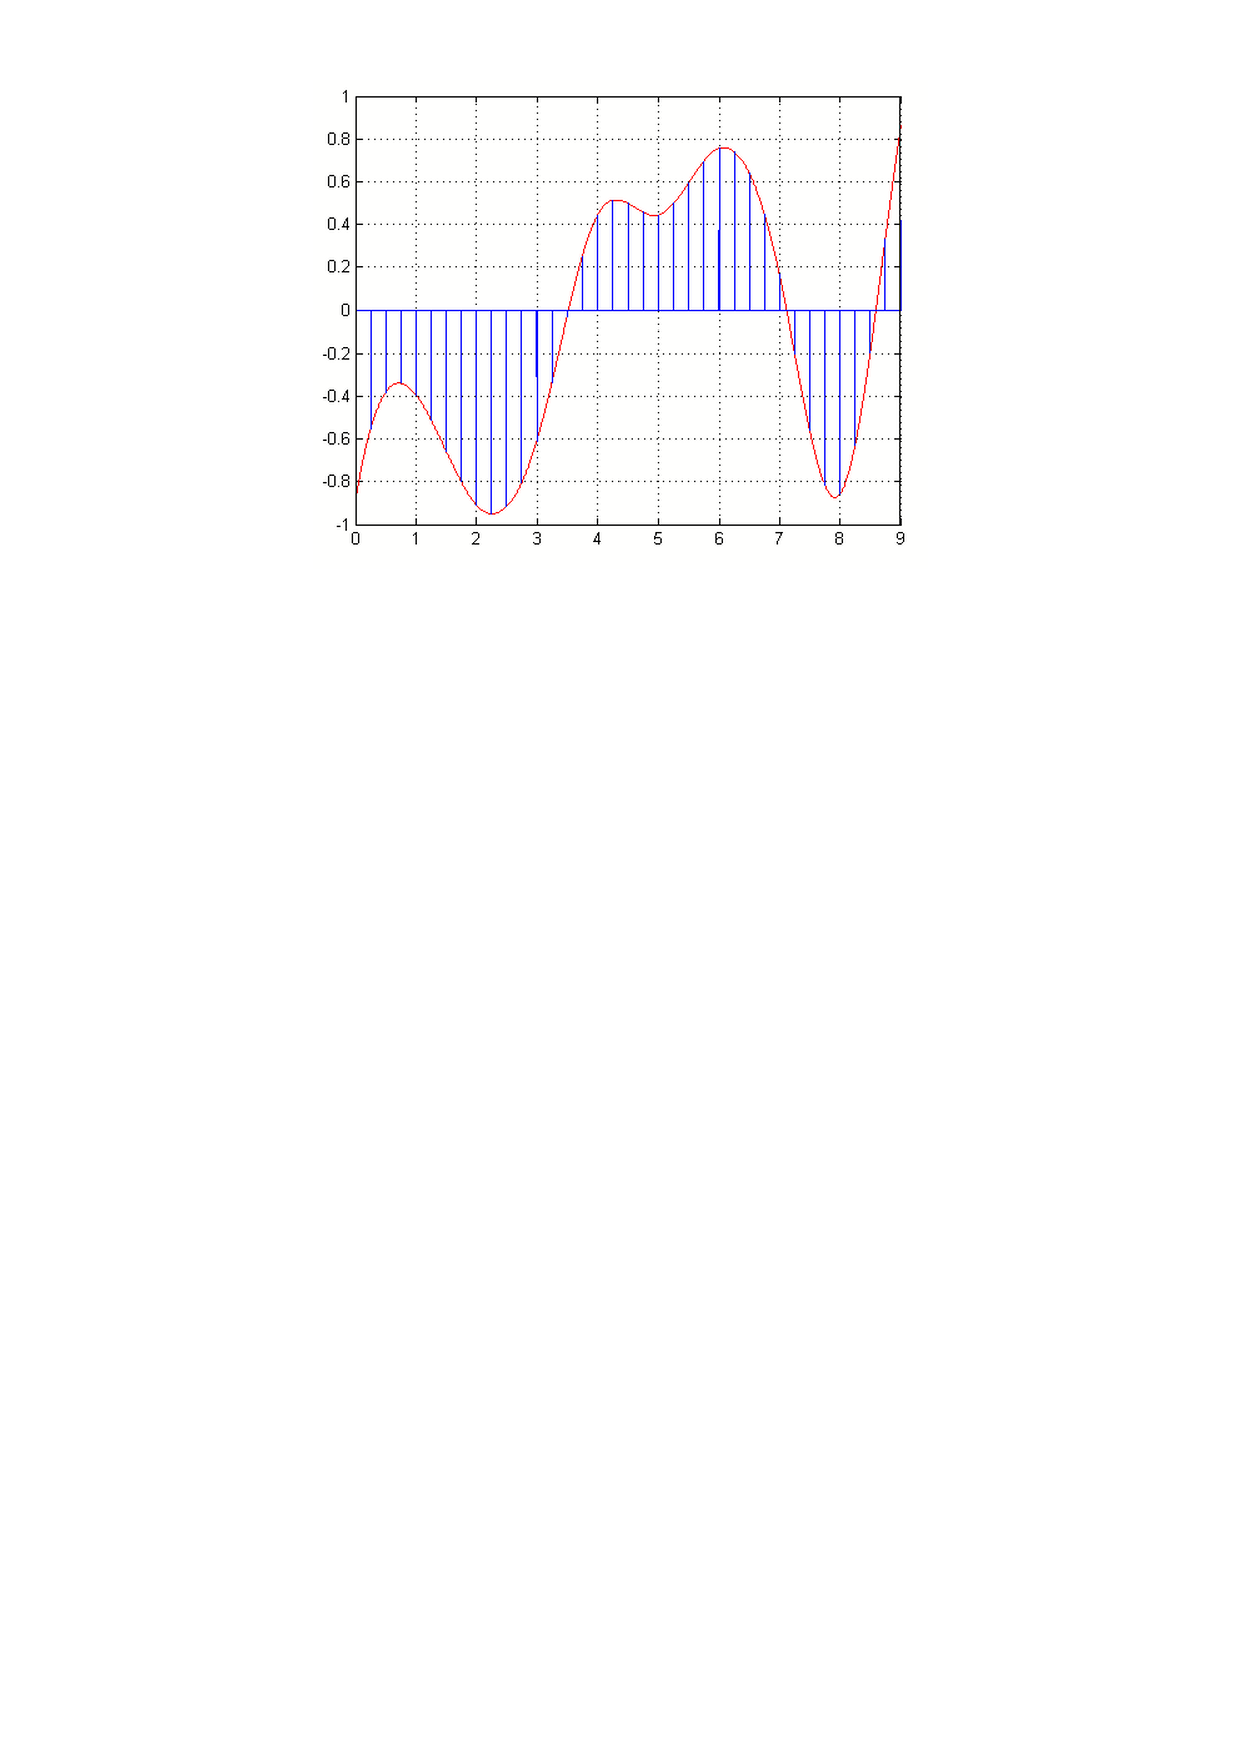
\includegraphics[width=0.6\textwidth]{sampling}\\
\end{figure}
\alert{$T$} the \alert{sampling period}. \alert{$f[n]= f(nT)$} are the samples of the signals.
The \alert{sampling frequency} \alert{$1/T$}.
\end{frame}


\begin{frame}
\frametitle{Band Limited functions}
\begin{definition}[Band Limited function]
A function $f \in L_2(\rset)$ is said to be  \alert{band limited} if there exists $B < \infty$ such that: $\TF f(\xi) = 0$ pour $\xi \not \in [-B,+B]$. We denote $\BL{B}$ the subspace of $f \in L_2(\rset)$ of functions satisfying $\TF f(\xi) = 0$ for (almost) all $\xi \not \in [-B,+B]$.
\end{definition}
\end{frame}


\begin{frame}
\frametitle{Periodizing the Fourier transform}
\only<1->{Let $T \leq 1/(2B)$ be the \alert{sampling period} and $1/T$ be the \alert{sampling frequency}.
Consider the periodic function $\xi \to \TF f(\xi)$ given by:
$$
F_T (\xi) = \sum_{n \in \zset} [\TF f] \left( \xi - \frac{n}{T} \right) \eqsp.
$$
}
\only<2>{$\xi \mapsto F_T(\xi)$ is periodic with period $1/T$}
\only<3>{The function  $F_T \in L_2{[-1/2T,1/2T]}$ can be expanded as a series function
\begin{equation*}
F_T (\xi) = \sum_{n \in \zset} c_n(F_T) \rme^{- \rmi 2 \pi \xi n T},
\end{equation*}
where $\{c_k(F_T)\}$, the Fourier coefficients are given by
\begin{equation*}
c_k(F_T) = T \int_{-1/(2T)}^{1/(2T)} F_T(\xi) \rme^{+ \rmi 2 \pi \xi k T} \rmd \xi\eqsp.
\end{equation*}
}
\end{frame}

\begin{frame}
\frametitle{Periodizing the Fourier transform}
The identity
\begin{equation*}
F_T (\xi) = \sum_{n \in \zset} c_n(F_T) \rme^{- \rmi 2 \pi \xi n T},
\end{equation*}
should be understood as a convergence of the partial sums
\begin{equation*}
F_{N,T}(\xi)= \sum_{k=-N}^N c_N(F_T) \rme^{- \rmi 2 \pi \xi n T} \eqsp,
\end{equation*}
toward $F_T$ in the topology induced by the norm $\|\cdot\|_2$  in $L_2([-1/(2T),1/(2T)])$:
$$
\lim_{N \to \infty} \int_{-1/(2T)}^{1/(2T)} |F_T(\xi) - F_{N,T}(\xi)|^2 \rmd \xi =0 \eqsp.
$$
\only<2>{The Parseval identity implies that $\sum_{n \in \zset} |c_n(F_T)|^2 < \infty$}.
\end{frame}

\begin{frame}
\frametitle{A key result}
\begin{itemize}
\item Since for all $T \leq 1/(2B)$, $[-B,+B] \subset [-1/(2T), 1/(2T)]$, then for all $\xi \in [-1/(2T),1/(2T)]$,
\alert{
$$F_T(\xi) = \TF f(\xi) $$
}
\item Therefore, the  Fourier coefficients $c_k(F_T)$ are given by:
\alert{
\begin{equation*}
c_k(F_T) = T \int_{-B}^{B} \TF f(\xi) \rme^{+ \rmi 2 \pi \xi k T} \rmd \xi= T f(kT)\eqsp.
\end{equation*}
}
\end{itemize}
\end{frame}



\begin{frame}
\frametitle{The Poisson Formula: Key result}
If $f \in \BL{B}$ then the \alert{discrete-time Fourier transform} (DTFT) of the sequence of samples $\{ f(nT), n \in \zset \}$
\[
T \sum_{n \in \zset} f(nT) \rme^{- \rmi 2 \pi \xi n T}
\]
is equal to the Fourier transform of the function $f$ periodized with a period $1/T$, a relation called the \alert{Poisson formula}
\begin{equation*}
\label{eq:FormuleSommatoirePoisson}
\sum_{n \in \zset} \TF f \left( \xi - \frac{n}{T} \right)  = T \sum_{n \in \zset} f(nT) \rme^{- \rmi 2 \pi \xi n T}\eqsp,
\end{equation*}
\only<2>{An amazing result: the DTFT is computable only from the knowledge of the samples $\{f(nT), n \in \zset\}$, whereas
the knowledge of $\TF f$ requires to evaluate the function at all time points
}
\only<3>{The DTFT is periodic with period $1/T$. Because of this periodicity, one may restrict the frequency
interval to just one-period, $[-1/2T,1/2T]$}
\end{frame}

%\begin{frame}
%\frametitle{Interpolation formula}
%\begin{itemize}
%\item \alert<1>{Multiply the Poisson formula
%\begin{equation*}
%\sum_{n \in \zset} \TF f \left( \xi - \frac{n}{T} \right)  = T \sum_{n \in \zset} f(nT) \rme^{- \rmi 2 \pi \xi n T}\eqsp,
%\end{equation*}
%by the indicator function $\1_{[-1/(2T),1/(2T)]}(\xi)$}
%\item \alert<2>{Use the identity $$\1_{[-1/(2T),1/(2T)]}(\xi) \TF f (\xi)= \1_{[-1/(2T),1/(2T)]}(\xi) F_T(\xi)$$}
%\end{itemize}
%
%\end{frame}

%\begin{frame}
%\frametitle{Interpolation formula}
%For all $\xi \in [-1/2T,+1/2T]$,
%$$
%\TF f (\xi) = T \sum_{n \in \zset} f(nT) \1_{[-1/(2T),1/(2T)]}(\xi) \rme^{- \rmi 2 \pi \xi n T} \eqsp.
%$$
%which should be understood as
%$$
%\lim_{N \to \infty} \int \left| \TF f(\xi)  - T \sum_{n =-N}^N f(nT) \1_{\left[-\frac{1}{2T},\frac{1}{2T}\right]}(\xi) \rme^{- \rmi 2 \pi
%    \xi n T}  \right|^2 \rmd \xi = 0 \eqsp.
%$$
%Since $\TFC$ is an isometry and $\TFC \TF f = f$ a.e.
%$$
%\lim_{N \to \infty} \int \left| f(t)  - T \sum_{n =-N}^N f(nT) \TFAC{\1_{\left[-\frac{1}{2T},\frac{1}{2T}\right]}(\xi) \rme^{+ \rmi 2 \pi
%    \xi n T}}(t) \right|^2 \rmd t = 0 \eqsp.
%$$
%\end{frame}
%
%\begin{frame}
%\frametitle{Interpolation formula}
%\begin{lemma}
%$$
%\TFAC{\xi \to \1_{[-1/(2T),1/(2T)]}(\xi) \rme^{+ \rmi 2 \pi \xi n T}}(x)= \frac{\sin\left( \frac{\pi}{T}(x - nT)\right)}{\pi(x-nT)}
%$$
%\end{lemma}
%
%
%\end{frame}

\begin{frame}
\frametitle{Interpolation formula}
\begin{theorem}[Nyquist theorem]
If $f \in \BL{B}$ and $T \leq 1/2B$ then
\alert{
\begin{equation*}
f(x) =_{\ltwo(\rset)} \sum_{n \in \zset} f(nT) s_T(x-nT)  \eqsp,
\end{equation*}
}
where $s_T$, is the cardinal-sine function
\alert{
$$
s_T(x) = \frac{\sin \left( \pi x/T\right) }{ \pi x/T}\eqsp.
$$
}
\end{theorem}
The condition  \alert{$T \leq 1/2B$} is the \alert{Nyquist condition}.
\end{frame}

\section{Another approach to sampling}
\begin{frame}
\frametitle{Why ?}
\begin{itemize}
\item Sampling theorem can be derived from another perspective, which is in some sense broader.
\item It acknowledges the fact that a function can be seen as a superposition if complex exponential (\alert{think !} this is the meaning of the Fourier synthesis formula...)
\item The approach starts by deriving the sampling theorem first for complex exponential, and then to extends the result to a (much) wider class of signals.
\end{itemize}
\end{frame}

\begin{frame}
\frametitle{Problem}
\begin{itemize}
\item Consider the function $s_{\xi_0}(x)= \rme^{2 \rmi \pi \xi_0 x}$, $\xi_0 \in \rset$. This function is neither in $\lone(\rset)$ or in $\ltwo(\rset)$, and therefore does not fit into the framework presented earlier.
\item A natural question is the following: under which conditions on the sampling period $T$ may we retrieve $s(x)$ from the its samples $\{s(nT), n \in \zset\}$.
\item Since $s_{\xi_0}(nT)= \rme^{2 \rmi \pi \xi_0 n T}$, we have
$$
s_{\xi_0}(nT)= s_{\xi_0 + k/T}(nT) \eqsp, \quad \text{for all $k,n \in \zset$}
$$
\item If $\xi_0 \in \ooint{-1/2T,1/2T}$ we can retrieve $s_{\xi_0}$ from its samples without error !
\end{itemize}
\end{frame}


\begin{frame}
\frametitle{A sampling theorem for complex exponential}
\begin{theorem}
For all $x \in \rset$ and  $\xi_0 \in \ooint{-1/2T,1/2T}$,
\[
\rme^{2 \rmi \pi \xi_0 x} = \sum_{n \in \zset} \rme^{2 \rmi \pi \xi_0 n T} s_T(x - nT) \quad s_T(x)= \frac{\sin\left( \pi x/T \right)}{\pi x /T}
\]
where the series in the RHS converges uniformly on $\ccint{-B,B} \subset \ooint{-1/2T,1/2T}$
\end{theorem}
\end{frame}


\begin{frame}
\frametitle{Sampling a finite sum of sinewaves}
\begin{itemize}
\item If $x \mapsto f(x)$ is a finite superposition of complex sinewaves,
\[
f(x)= \sum_{k=1}^M \gamma_k \rme^{2 \rmi \nu_k x}
\]
where $\{\gamma_k\}_{k=1}^M \in \cset$ and $\{ \nu_k \}_{k=1}^M \subset \ooint{-1/2T,1/2T}$, then the Nyquist formula holds
\[
f(x)= \sum_{k=-\infty}^{\infty}  f(kT) s_T(x - kT)
\]
\end{itemize}
\end{frame}

\begin{frame}
\frametitle{Decomposable signals}
\begin{itemize}
\item This can be extended to any function $f$ which can be written as
\[
f(x)= \int_{-B}^B \rme^{2 \rmi \pi \xi x} \mu(\rmd x)
\]
where $\mu$ is a signed measure on $\ccint{-B,B}$ as soon as $B < 1/2T$.
\end{itemize}
\end{frame}


\section{Frequency resolution and windowing}

\begin{frame}
\frametitle{From theory to practice}
\begin{itemize}
\item Even though $T\sum_{k=-\infty}^{\infty} f(kT) \rme^{-\rmi 2 \pi \xi kT}$ is the closest approximation  of $\TF f$ that we can achieve digitally, it is still not computable because generally it requires an \alert{infinite number of samples}.
\item To make it computable, we must make a \alert{second approximation}, keeping only a \alert{finite number} of samples $\{ f(kT), 0\leq k \leq L-1\}$ (assuming a \alert{causal} signal).
\item In terms of the times samples, the \alert{time windowed version} is given by
\[
T \sum_{k=0}^{L-1} f(kT) \rme^{- \rmi 2 \pi \xi kT}
\]
\end{itemize}
\end{frame}

\begin{frame}
\frametitle{Normalized frequency}
\begin{itemize}
\item It is customary to define the \alert{normalized} frequency as \alert{$ \lambda = \xi/ \xi_s$}, where \alert{$\xi_s= 1/T$} is the sampling frequency.
\item Expressed in terms of the normalized frequency $\lambda$, the discrete time Fourier transform is given by
\[
\lambda \mapsto T \sum_{k=-\infty}^{\infty} f(kT) \rme^{- \rmi 2 \pi k \lambda}
\]
which is periodic with period $1$. It is customary to represent this function on the interval $\ccint{-1/2,1/2}$.
\item It is sometimes more appropriate to work with the \alert{normalized pulsation} \alert{$\omega= 2 \pi \lambda$}.
\item In the sequel we set conventionally $T=1$
\end{itemize}
\end{frame}

\begin{frame}
\frametitle{From theory to practice}
\begin{itemize}
\item The windowed signal may be thought of as an \alert{infinite sequence} which is zero outside the range of the window and agrees with the original one within the window.
\item To express this mathematically, we define the \alert{rectangular} window of length $L$:
\[
w(n) =
\begin{cases}
1 \eqsp & n \in \{0,\dots,L-1\} \\
0 &  \text{otherwise}
\end{cases}
\]
\item The Discrete time Fourier transform of the windowed signal $\{ w(n) f(n), n=0,\dots,L-1\}$ is given by
\[
F_L(\omega)= \sum_{k=0}^{L-1} w(k) f(k) \rme^{-\rmi \omega k} \eqsp.
\]
%\item As the window length $L$ increases, the windowed DTFT becomes a better approximation of the DTFT
%\[
%F(\omega) = \sum_{k=-\infty}^{\infty} f(k) \rme^{-\rmi \omega k} \eqsp,
%\]
%and is computable for any value of the pulsation $\omega$.
\end{itemize}
\end{frame}

\begin{frame}
\frametitle{Windowing effect}
\begin{itemize}
\item In general, the windowing process has two major effects:
\begin{enumerate}
\item First, it reduces the \alert{frequency resolution} of the computed spectrum, in the sense that the \alert{smallest resolvable frequency} difference is limited by the length of the data record. This is linked with the \alert{uncertainty principle.}
 \item Second, it introduces \alert{spurious} high-frequency components into the spectrum, which are caused by the sharp clipping of the signal at the left and right ends of the rectangular window. This effect is referred to as \alert{frequency leakage.}
\end{enumerate}
\item Both effects can be understood by deriving the precise effect of windowing on the Discrete Tile Fourier Transform.
\end{itemize}
\end{frame}

\begin{frame}
\frametitle{Convolution}
\begin{itemize}
\item Recall that $f(n)$ is the $n$-th Fourier coefficient of the $\pi$-periodic function $F(\omega)$
\[
f(n) = \frac{1}{2 \pi} \int_{-\pi}^{\pi} F(\omega') \rme^{+ \rmi \omega' n} \rmd \omega'
\]
\item Evaluate the DTFT of the windowed sequence $\{ w(n) x(n), n \in \nset\}$:
\begin{align*}
\sum_{n=-\infty}^{\infty} x(n) w(n) \rme^{-\rmi \omega n} &= (2 \pi)^{-1} \sum_{n=-\infty}^{\infty} w(n) \int_{-\pi}^{\pi} X(\omega') \rme^{-\rmi (\omega-\omega') n} \rmd \omega' \\
&= (2\pi)^{-1} \int_{-\pi}^\pi X(\omega') W(\omega - \omega') \rmd \omega'
\end{align*}
where $W(\omega)$ is the DTFT of the window
\[
W(\omega)= \sum_{k=0}^{L-1} w(n) \rme^{-\rmi \omega n} \eqsp.
\]
\end{itemize}
\end{frame}

\begin{frame}
\frametitle{Fourier transform of a rectangular window}
\begin{itemize}
\item The DTFT of the recatngular window is given by
\[
\sum_{k=0}^{L-1} \rme^{-\rmi \omega k}= \frac{\sin(\omega L/2)}{\sin(\omega/2)} \rme^{- \rmi \omega (L-1)/2}
\]
\item The function has a maximum at $0$ which is equal to $L$ and is $\pi$ periodic.
\end{itemize}
\end{frame}

\begin{frame}
\begin{figure}
  \centering
  % Requires \usepackage{graphicx}
  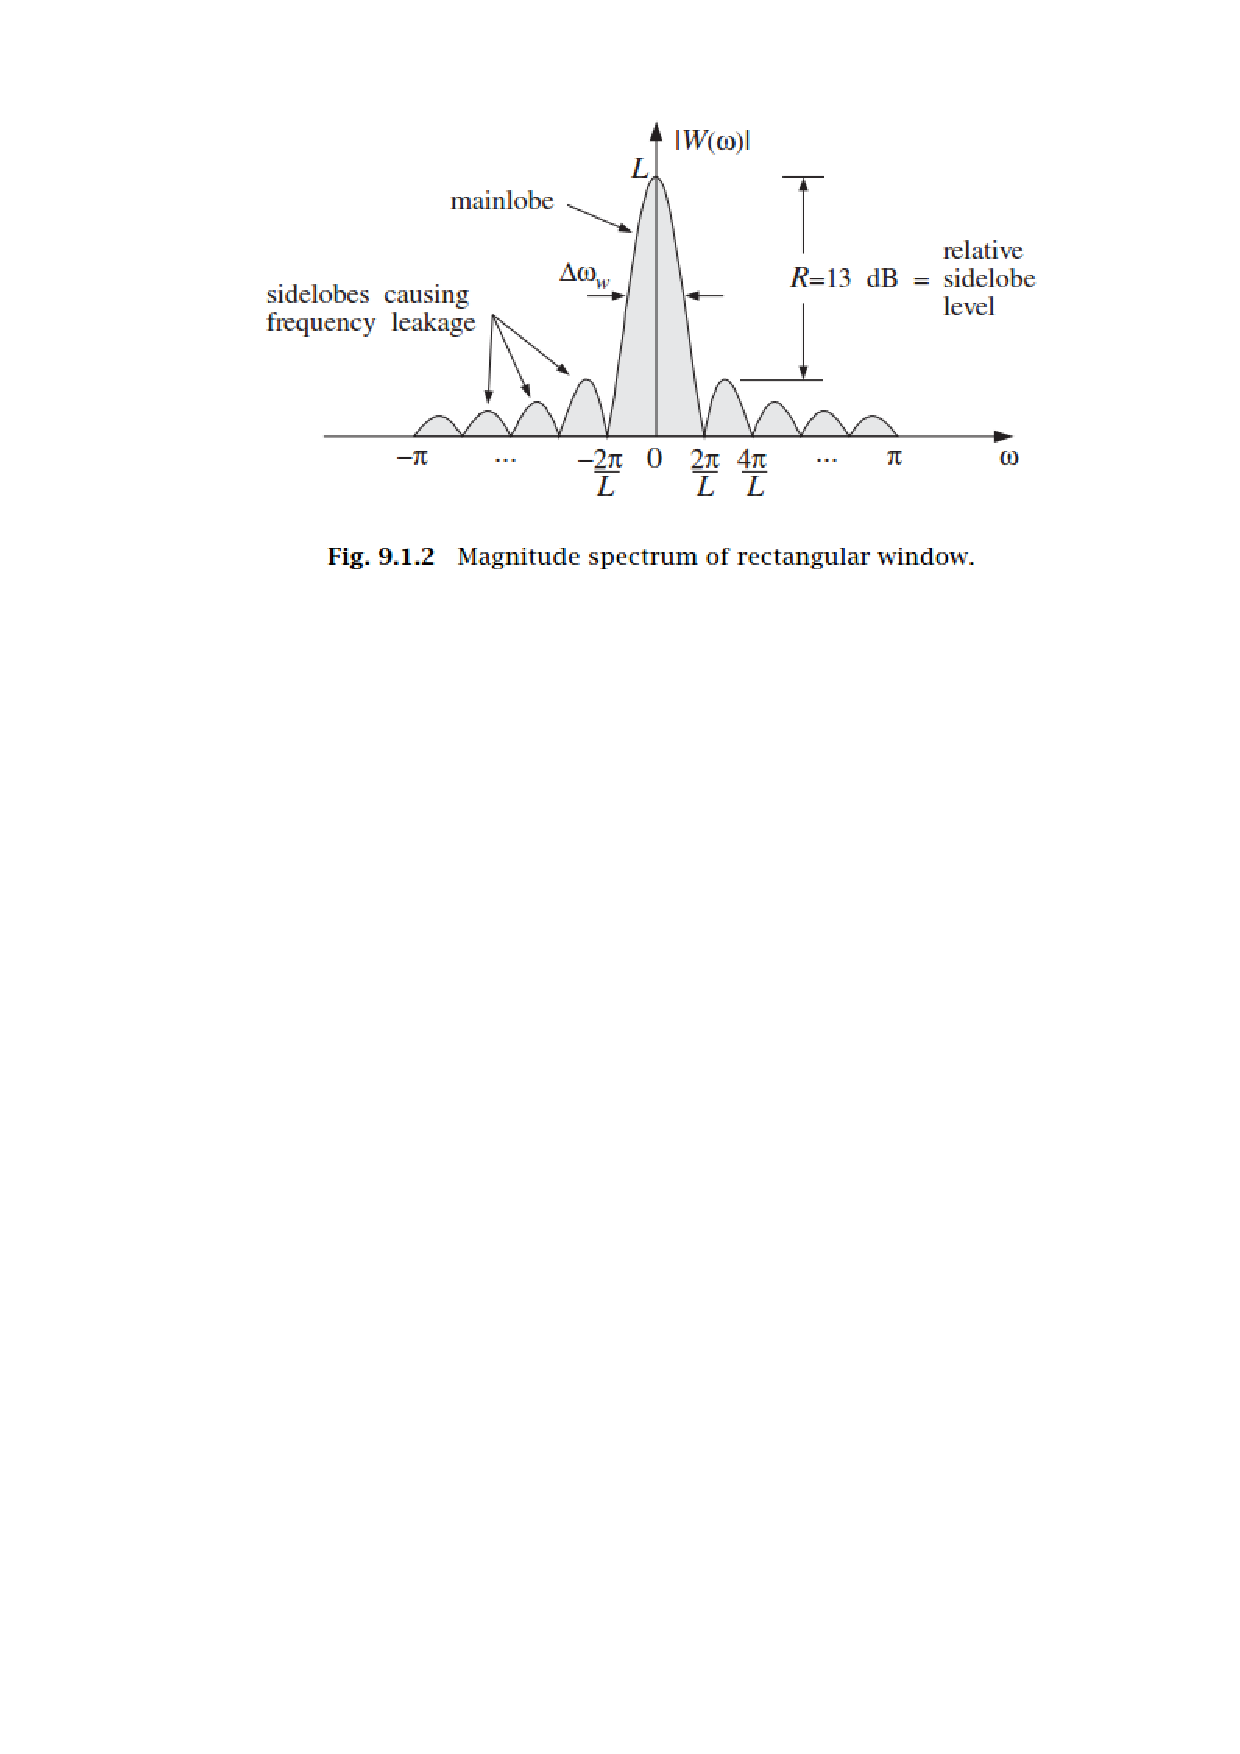
\includegraphics[width=0.7\textwidth]{rectangularw}\\
\end{figure}
\end{frame}

\begin{frame}
\begin{figure}
  \centering
  % Requires \usepackage{graphicx}
  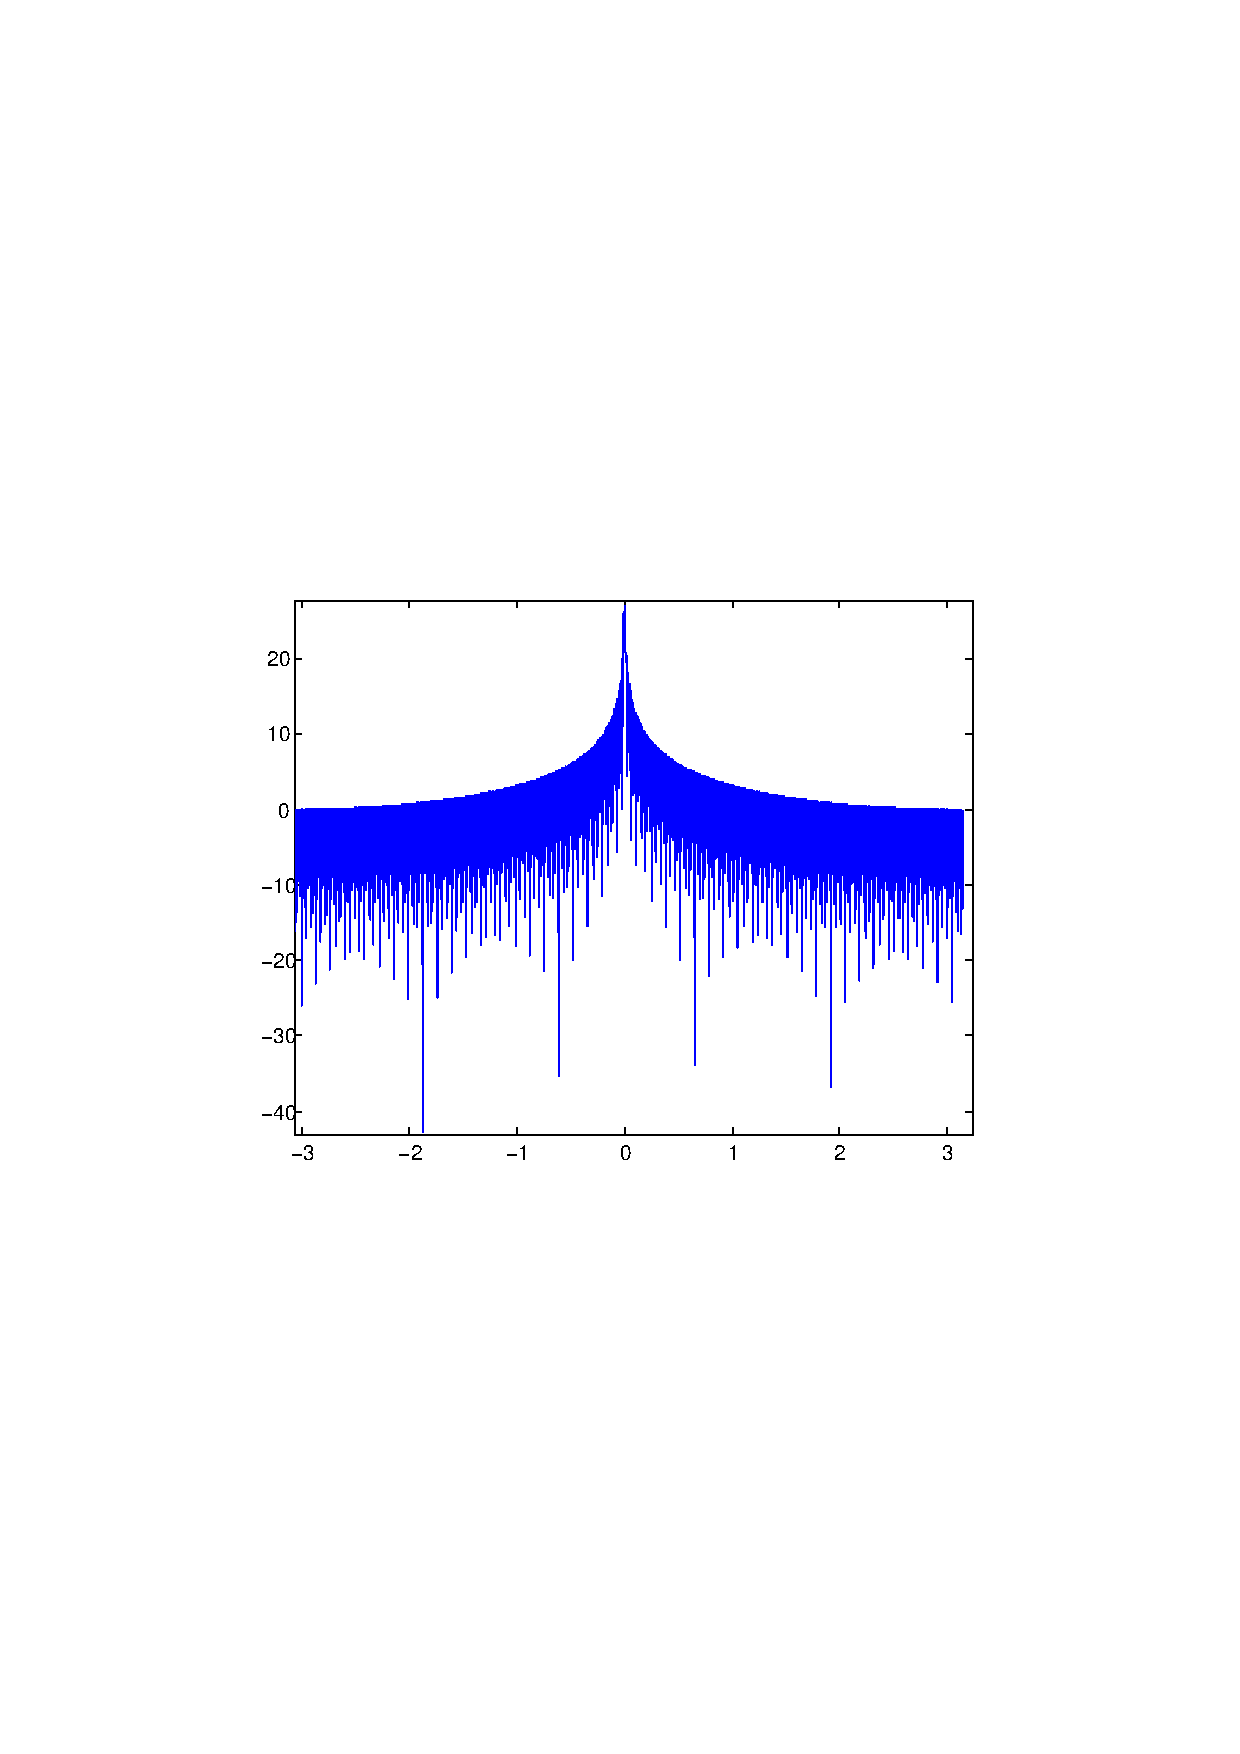
\includegraphics[width=0.7\textwidth]{rectangularw256}\\
\end{figure}


\end{frame}

\begin{frame}
\frametitle{Mainlobes and sidelobes}
\begin{itemize}
\item It consists of a \alert{main lobe} of height $L$ and base width $4\pi/L$ centered at $\omega=0$, and several smaller \alert{sidelobes}.
\item The sidelobes are between the zeros of $W(\omega)$ , which are the zeros of the numerator $\sin(\omega L/2)=0$, that is, $\omega=2\pi k/L$, for $k=\pm 1, \pm 2,\ \ldots$ (with $k=0$ excluded).
\item The mainlobe peak at $0$ dominates the spectrum, because $w(n)$ is essentially a low-pass  signal, except when it cuts off at its endpoints.
\item The higher frequency components that have `leaked'' away from $0$ and lie under the sidelobes represent the sharp transitions of $w(n)$ at the endpoints.
\end{itemize}
\end{frame}

\begin{frame}
\frametitle{Mainlobes and sidelobes}
\begin{itemize}
\item  For simplicity, we  define the width of the mainlobe  to be half the base width, that is, in units of radians per sample:
$$
\Delta\omega_{w}=\frac{2\pi}{L} \quad \text{(rectangular window width)}
$$
\item In units of Hz, it is defined through $\Delta\omega_{w}=2\pi\Delta \xi_{w}/\xi_{s}$:
$$
\Delta \xi_{w}=\frac{\xi_{s}}{L}=\frac{1}{LT}=\frac{1}{T_{L}}\
$$
\item The mainlobe width $\Delta \xi_{w}$ determines the \alert{frequency resolution limits} of the windowed spectrum.
\begin{itemize}
\item As $L$ increases, the height of the mainlobe increases and its width becomes narrower, getting more concentrated around 0.
\item However, the height of the sidelobes also increases, but \alert{relative} to the mainlobe height, it remains approximately the same and about 13 dB down.
\end{itemize}
\end{itemize}
\end{frame}

\begin{frame}
\frametitle{Better analysis windows}
\begin{itemize}
\item Windows are commonly used for spectral analysis. They have the desirable properties that
\begin{itemize}
\item their Fourier transforms is concentrated around $\omega=0$,
\item they have \alert{simple functional forms} that allow them to be computed esasily.
\end{itemize}
\item \alert{Examples}
\begin{enumerate}
\item \alert{Bartlett} $w(n)= (2 n/L) \indi{n \leq L/2} + (2 - 2 n /L) \indi{n > L/2}$, for $ n =0,\dots, L-1$.
\item \alert{Hanning}  $w(n)= 0.5 - 0.5 \cos(2 \pi n/L)$, for $ n =0,\dots, L-1$.
\item \alert{Hamming} $w(n)= 0.54 - 0.46 \cos(2 \pi n /L)$, for $ n =0,\dots, L-1$.
\item \alert{Blackman} $w(n)= 0.42 - 0.5 \cos(2 \pi n/L) + 0.08 \cos(4 \pi n /L)$, for $n=0, \dots, L-1$.
\end{enumerate}
\end{itemize}
\end{frame}

\begin{frame}
\frametitle{Analysis windows}
\begin{figure}
  \centering
  % Requires \usepackage{graphicx}
  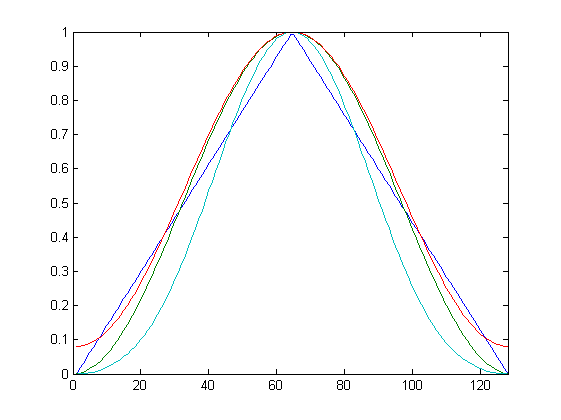
\includegraphics[width=0.7\textwidth]{window}
  \caption{Bartlett, Hanning, Hamming and Blackman windows}
\end{figure}
\end{frame}

\begin{frame}
\frametitle{Discrete-time Fourier transform of analysis windows}
\begin{figure}
  \centering
  % Requires \usepackage{graphicx}
  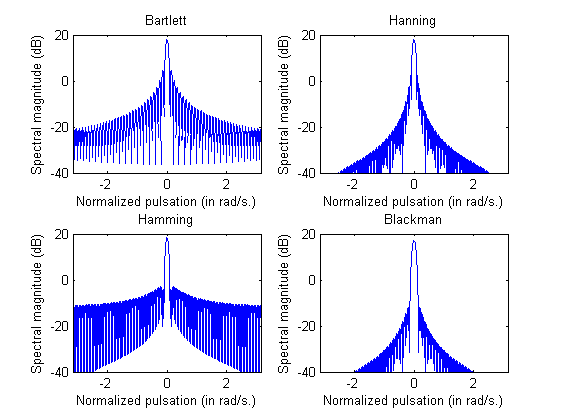
\includegraphics[width=0.7\textwidth]{spectralwindow}
  \caption{Bartlett, Hanning, Hamming and Blackman windows}
\end{figure}
\end{frame}


\section{The Discrete Fourier Transform: definitions and illustration}
\begin{frame}
\frametitle{Definition}
\begin{itemize}
\item The $N$-point \alert{Discrete Fourier Transform} of a length-$L$ signal is defined to be the DTFT evaluated at $N$ equally spaced frequencies over the full Nyquist interval, $ 0\leq\omega\leq 2\pi$. These \alert{DFT frequencies} are defined in radians per sample as follows:
$$
\omega_{k}=\frac{2\pi k}{N}\ k=0,1,\ \ldots,\ N-1
$$
or, in Hz
$$
h\ =\frac{kf_{s}}{N}\ k=0,1,\ \ldots,\ N-1
$$
\item Thus, the $N$-point DFT will be, for $k=0,1,\ \ldots$ , $N -1$:
\[
F(\omega_k)= \sum_{n=0}^{L-1} f(n) \rme^{-\rmi \omega_k n}
\]
\end{itemize}
\end{frame}

\begin{frame}
\frametitle{zero-padding}
\begin{itemize}
\item In principle, the two lengths $L$ and $N$ can be specified \alert{independently} of each other: $L$ is the number of \alert{times  samples} in the data record and can even be infinite; $N$ is the number of \alert{frequencies} at which we choose to evaluate the DTFT.
\item Most discussions of the DFT assume that $L=N$. The reason for this will discussed later.
\item If $L<N$, we can \alert{pad} $N-L$ zeros at the end of the data record to make it of length $N$.
\item If $L>N$, we may reduce the data record to length $N$ by \alert{wrapping} it modulo-$N$
\end{itemize}
\end{frame}


\begin{frame}
\frametitle{Physical versus computation resolution}
\begin{itemize}
\item The bin width $2 \pi / N$ represents (in normalized frequency) the spacing between the DFT frequencies at which the DFT is computed.
\item It \alert{should not} be confused with the \alert{frequency resolution width} which is linked with the analysis window (which is roughly proportional to the inverse of the window length $2 \pi / L$), which refers to the minimum \alert{resolvable} frequency separation between
    sinusoidal components.
\item To avoid confusion, we will refer to $2 \pi /L$ as the \alert{physical resolution} and $2 \pi / N$ as the \alert{computational resolution}.
\end{itemize}
\end{frame}

\begin{frame}
\frametitle{Physical / computational resolution}
\begin{figure}
  \centering
  % Requires \usepackage{graphicx}
  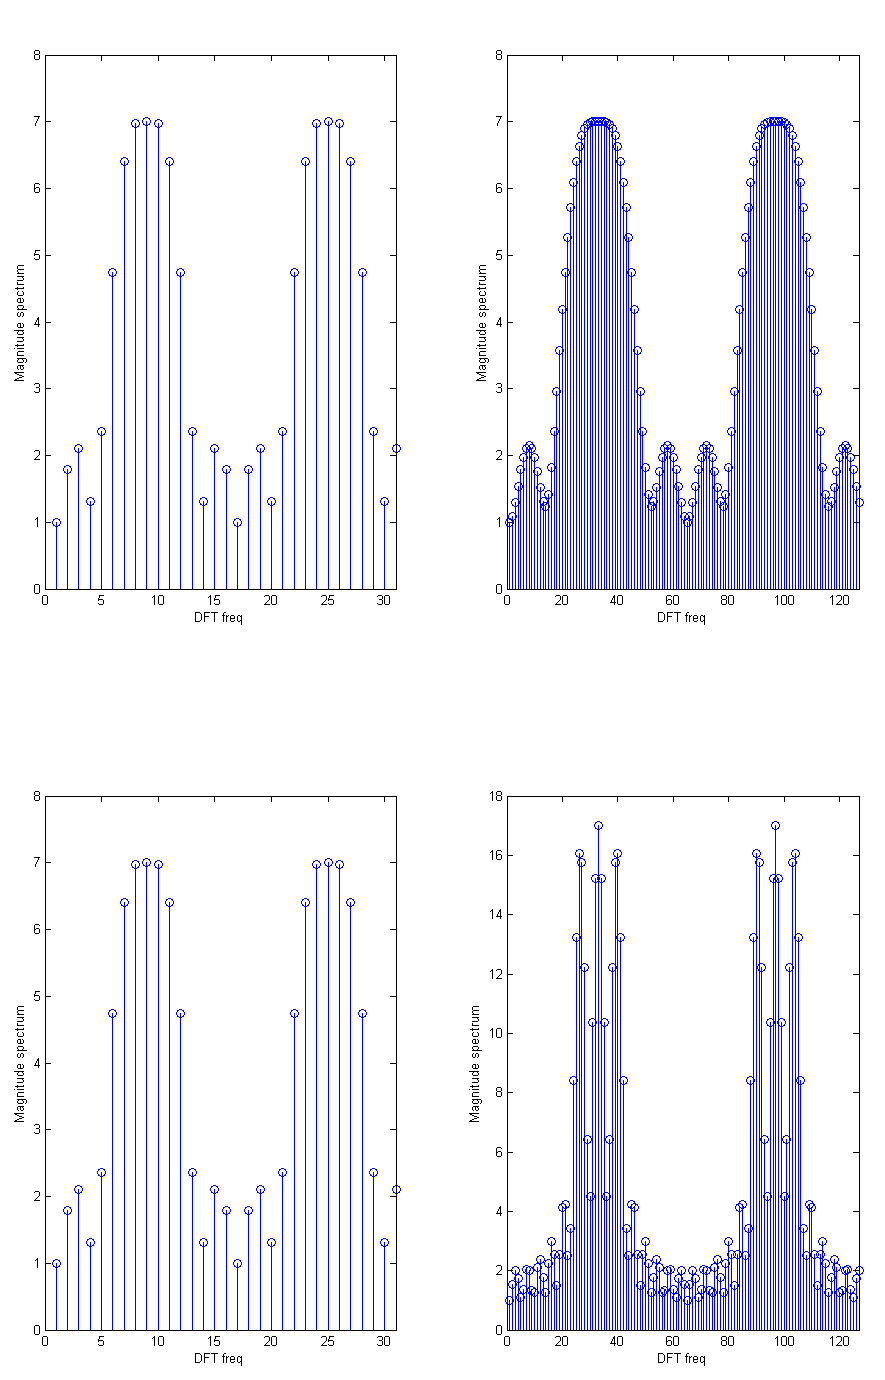
\includegraphics[width=0.4\textwidth]{3sinewaves.png}\\
\end{figure}
\end{frame}


\begin{frame}
\frametitle{Speech signal}
\begin{figure}
  \centering
  % Requires \usepackage{graphicx}
  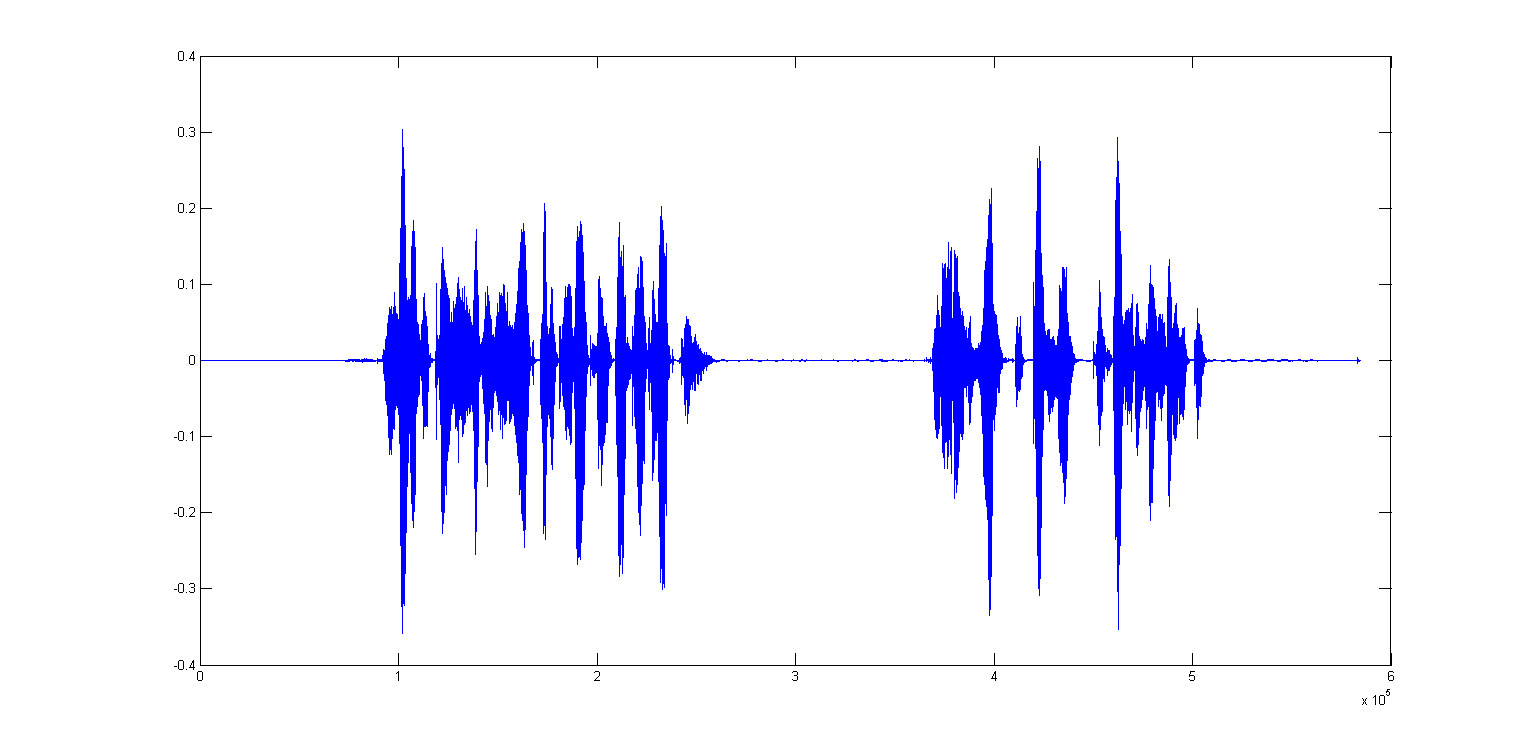
\includegraphics[width=0.8\textwidth]{speech}
\end{figure}
\end{frame}

\begin{frame}
\frametitle{Speech signal: extract}
\begin{figure}
  \centering
  % Requires \usepackage{graphicx}
  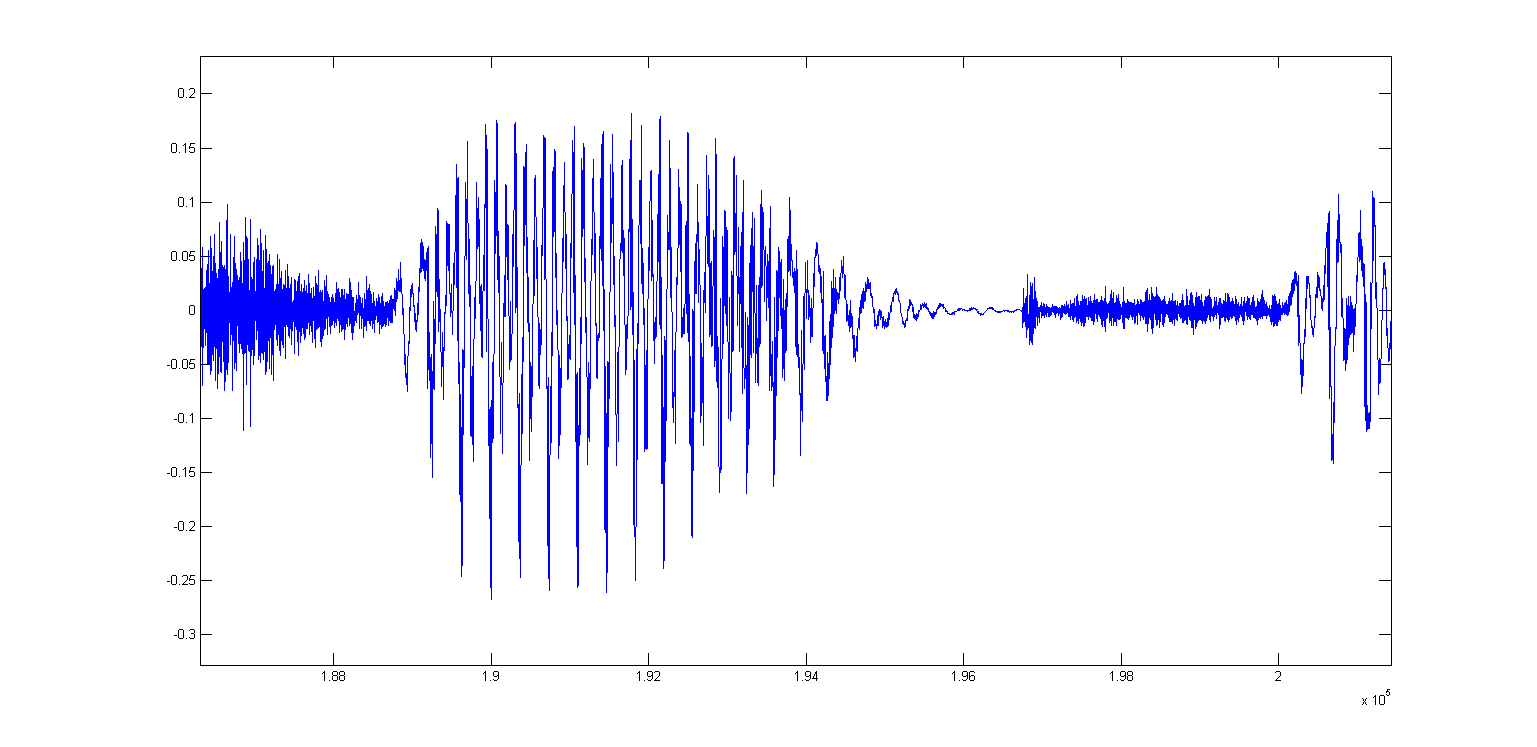
\includegraphics[width=0.8\textwidth]{speech-extract}
\end{figure}
\end{frame}


\begin{frame}
\frametitle{Speech signal: extract}
\begin{figure}
  \centering
  % Requires \usepackage{graphicx}
  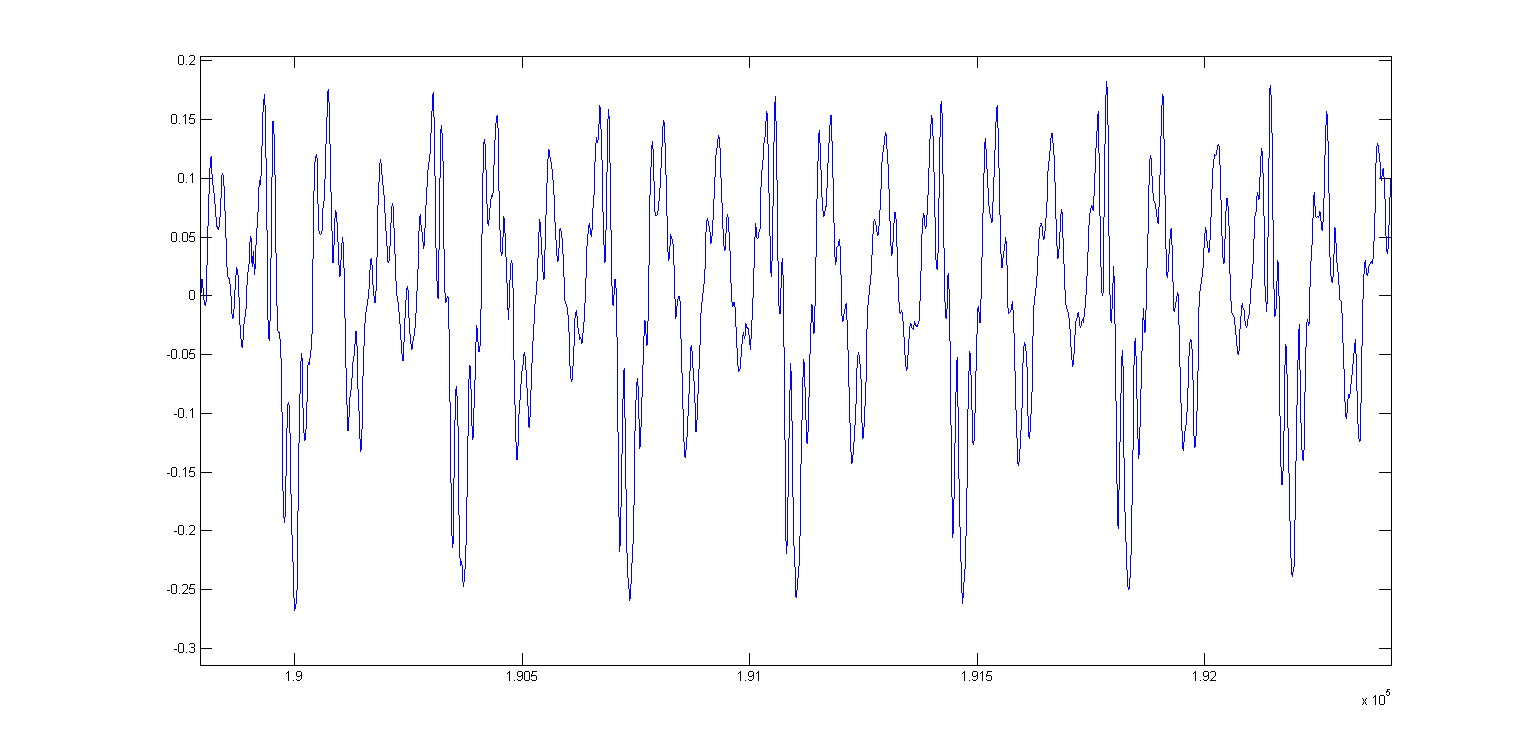
\includegraphics[width=0.8\textwidth]{speech-extract-1}
  \caption{Sampling frequency: 48kHz; Sampling period: 20.8 $\mu$sec; period: 371 samples; pitch= 129 Hz }
\end{figure}
\end{frame}


\begin{frame}
\frametitle{Speech signal: windowing}
\begin{figure}
  \centering
  % Requires \usepackage{graphicx}
  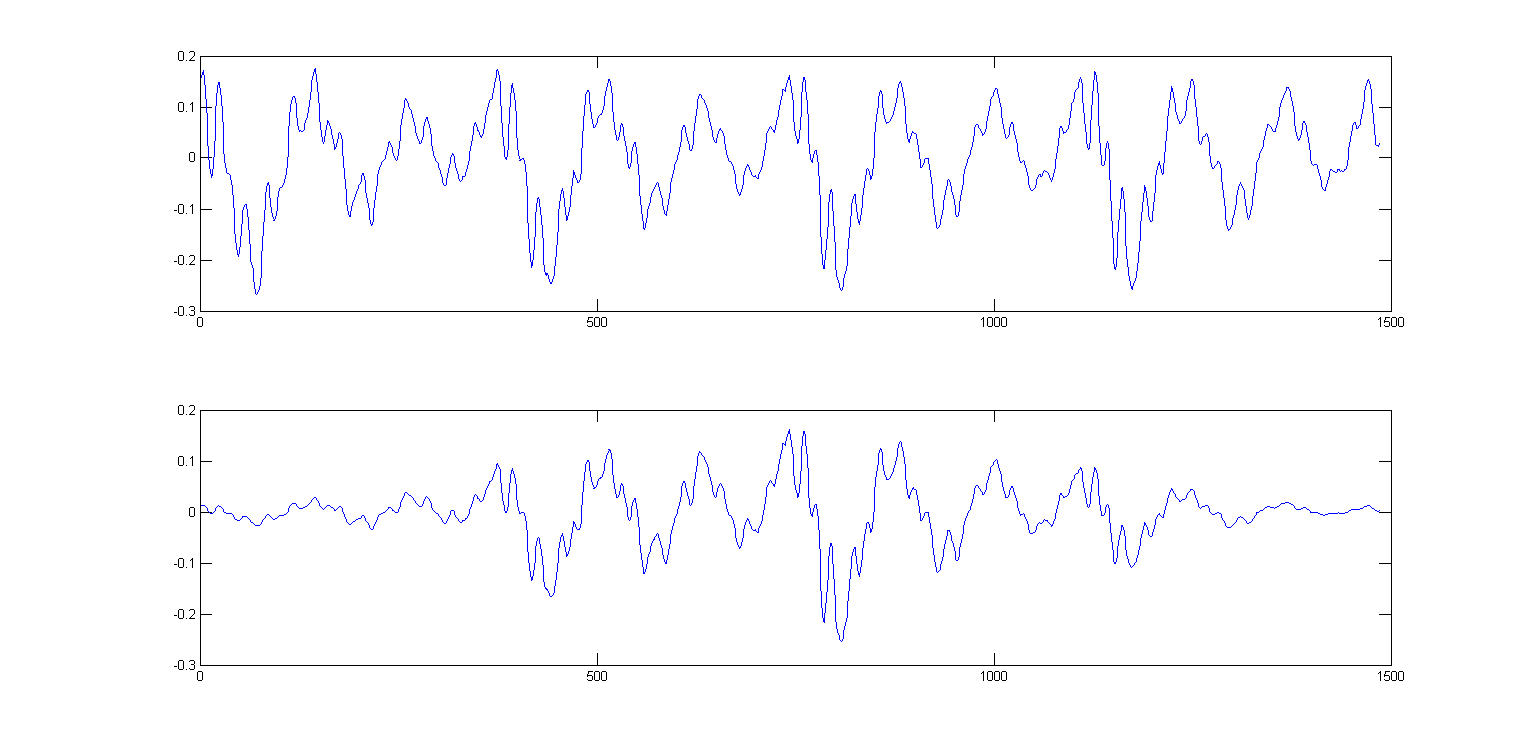
\includegraphics[width=0.8\textwidth]{speech-extract-windowed}
  \caption{Sampling frequency: 48kHz; Sampling period: 20.8 $\mu$sec; period: 371 samples; pitch= 129 Hz }
\end{figure}
\end{frame}


\begin{frame}
\frametitle{Speech signal: physical resolution}
\begin{figure}
  \centering
  % Requires \usepackage{graphicx}
  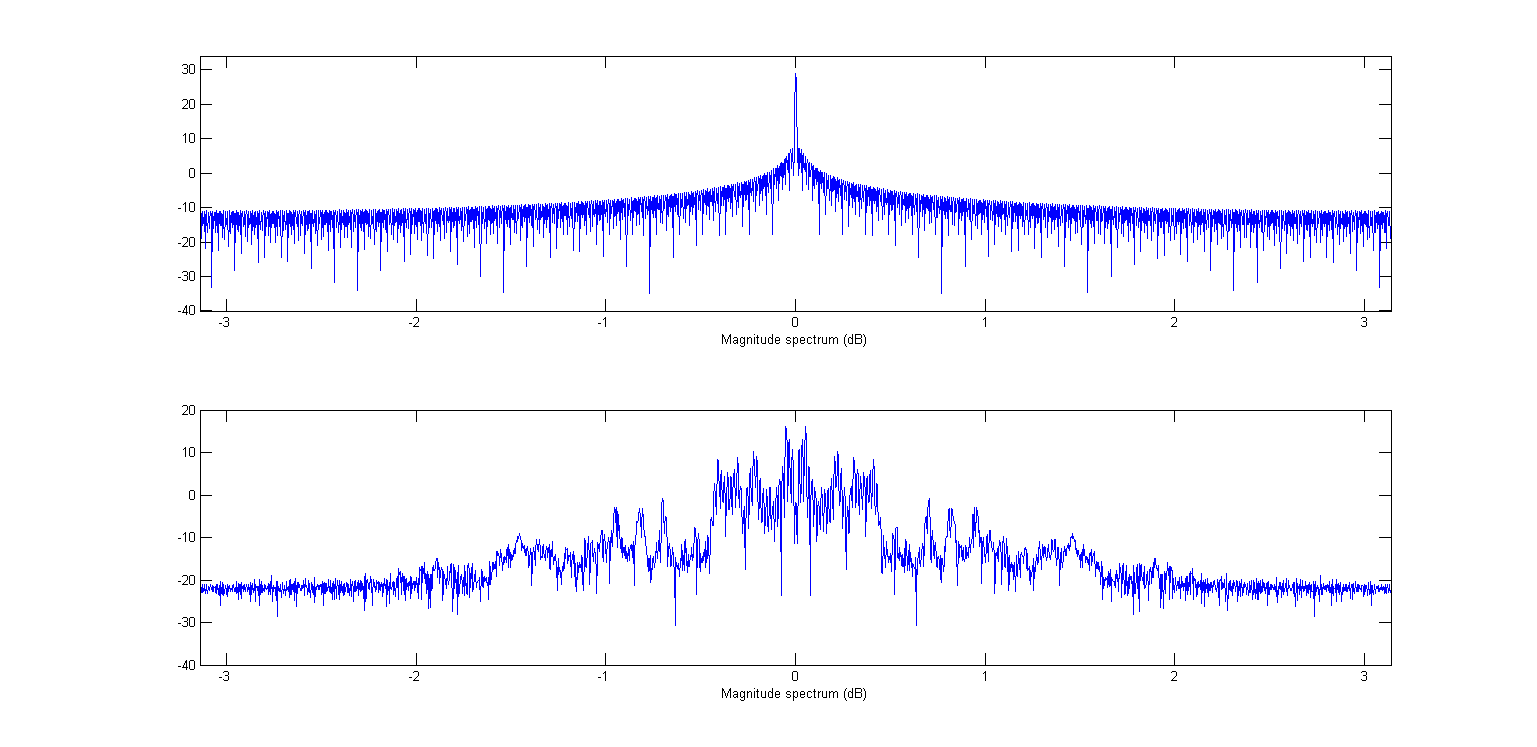
\includegraphics[width=0.8\textwidth]{speech-spectrum}
  \caption{Sampling frequency: 48kHz; Sampling period: 20.8 $\mu$sec; period: 371 samples; pitch= 129 Hz }
\end{figure}
\end{frame}

\begin{frame}
\frametitle{Speech signal: physical resolution}
\begin{figure}
  \centering
  % Requires \usepackage{graphicx}
  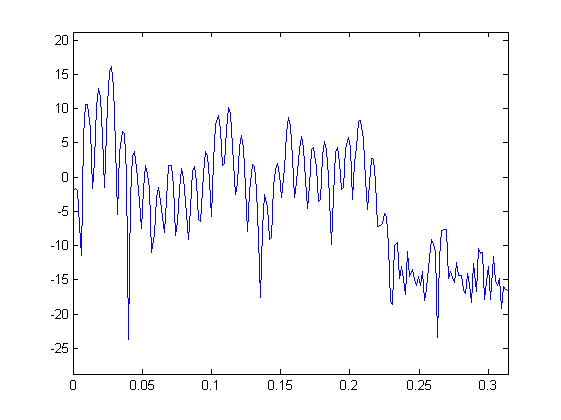
\includegraphics[width=0.8\textwidth]{speech-spectrum-extract}
  \caption{Sampling frequency: 48kHz; Sampling period: 20.8 $\mu$sec; period: 371 samples; pitch= 129 Hz }
\end{figure}
\end{frame}




\section{Discrete Fourier Series of a periodic sequence}
\begin{frame}
\frametitle{Discrete periodic sequences}
\begin{itemize}
\item Consider a sequence $\{ \tilde{x}(n), n \in \zset \}$ that is \alert{periodic} with period $N$, \ie\ for all $n$ and $r$,
\[
\tilde{x}(n)= \tilde{x}(n + rN) \eqsp.
\]
\item As with continuous-time periodic signals, such a sequence can be represented by a Fourier series corresponding to a sum of \alert{harmonically} related complex exponentials,
%\ie\ complex exponentials with frequencies that are \alert{integer multiples of the fundamental frequency}, $2 \pi /N$,
\[
\tilde{x}(n)= \frac{1}{N} \sum_{k \in \zset} \tilde{X}(k) \rme^{\rmi (2 \pi/ N) k n}
\]
\item Denoting $e_k: n \mapsto e_k(n)= \rme^{\rmi (2 \pi / N) n k}$ these complex exponentials, the periodic discrete time signal $\tilde{x}$ may be decomposed as
\[
\tilde{x}= \frac{1}{N} \sum_{k \in \zset} \tilde{X}(k) e_k
\]
\end{itemize}
\end{frame}

\begin{frame}
\frametitle{Discrete periodic sequences}
\begin{itemize}
\item  The Fourier series representation of a continuous-time periodic signal generally requires infinitely many harmonically related complex exponentials.
\item The Fourier series of any discrete time-signal with period $N$ requires only $N$ harmonically related complex exponentials since 
\[
e_{k + \ell N}(n)= e_k(n) \quad \text{for all $k, \ell \in \zset$} \eqsp.
\]
\item Consequently the set of $N$ periodic complex exponentials $\{e_0, e_1, \dots, e_{N-1}\}$ defines all the distinct periodic
exponentials and
\[
\tilde{x}(n) = \frac{1}{N} \sum_{k=0}^{N-1} \tilde{X}(k) e_k(n) \eqsp, \quad e_k: n \mapsto e_k(n)= \rme^{\rmi (2 \pi / N)n k}
\]
\end{itemize}
\end{frame}

\begin{frame}
\frametitle{Orthogonality}
\begin{itemize}
\item To obtain the sequence of Fourier series coefficients $\tilde{X}(k)$ from the periodic sequence $\tilde{x}$, we exploit the orthogonality of the set of complex exponentials $\{e_j\}_{j=0}^{N-1}$
\time Note indeed that
\[
\sum_{n=0}^{N-1} \tilde{x}(n) \rme^{-\rmi (2 \pi/N) r n} = \sum_{n=0}^{N-1} \frac{1}{N} \sum_{k=0}^{N-1} \tilde{X}(k) \rme^{\rmi (2 \pi/N) (k-r)n}
\]
\item After exchanging the order of summations, we obtain
\[
\sum_{n=0}^{N-1} \tilde{x}(n) \rme^{-\rmi (2 \pi/N) r n} = \sum_{k=0}^{N-1} \tilde{X}(k) \left[ \frac{1}{N} \sum_{n=0}^{N-1} \rme^{\rmi (2 \pi/N) (k-r) n} \right]
\]
\end{itemize}
\end{frame}

\begin{frame}
\frametitle{Orthogonality}
\begin{itemize}
\item The following identity expresses the orthogonality of the complex exponentials:
$$
\frac{1}{N}\sum_{n=1}^{N-1}\rme^{\rmi(2\pi/N)(k-r)n}=
\begin{cases}
1, k-r= mN, &\quad \text{$m$ an integer} \\
0 & \text{otherwise}
\end{cases}
$$
\item \alert{Conclusion}
$$
\sum_{n=0}^{N-1}\tilde{x}[n] \rme^{-\rmi(2\pi/N)r n}=\tilde{X}[r].
$$
\end{itemize}
\end{frame}

\begin{frame}
\frametitle{DFT coefficients properties}
\begin{itemize}
\item the sequence $\tilde{X}[k]$ is periodic with period $N$, \ie\, for any integer $k$:
\begin{align*}
\tilde{X}[k+N] &=\sum_{n=0}^{N-1}\tilde{x}(n) \rme^{-\rmi (2\pi/N)  (k+N) n} \\
&=\left(\sum_{n=0}^{N-1}\tilde{x}(n) \rme^{-\rmi(2\pi/N)k n} \right) \rme^{-\rmi 2\pi n}=\tilde{X}[k]
\end{align*}
\item An advantage of interpreting the Fourier series coefficients $\tilde{X}[k]$ as a periodic sequence is that there is then a \alert{duality} between the \alert{time} and \alert{frequency domains} for the Fourier series representation of periodic sequences.
\end{itemize}
\end{frame}

\begin{frame}
\frametitle{Analysis-Synthesis}
\[
\tilde{X}(k)= \sum_{n=0}^{N-1} x(n) \rme^{-\rmi (2 \pi/N) kn} \quad \tilde{x}(n)= \frac{1}{N} \sum_{k=0}^{N-1} \tilde{X}(k) \rme^{\rmi (2 \pi/N) k n}
\]
are an analysis-synthesis pair and will be referred to as the \alert{discrete Fourier series} (DFS) representation of a periodic sequence.\\
\bigskip
For convenience in notation, these equations are often written in terms of the complex quantity
\alert{$W_{N}= \rme^{-\rmi(2\pi/N)}$} and the DFS analysis-synthesis pair is expressed as follows:
\begin{align*}
&\alert{\text{Analysis\ equation}}:\ \tilde{X}[k]=\sum_{n=0}^{N-1}\tilde{x}[n]W_{N}^{kn} \\
&\alert{\text{Synthesis\ equation}}:\ \tilde{x}[n]=\frac{1}{N}\sum_{k=0}^{N-1}\tilde{X}[k]W_{N}^{-kn}
\end{align*}
\end{frame}


\begin{frame}
\frametitle{Linearity}
Consider two periodic sequences $\tilde{x}_{1}[n]$ and $\tilde{x}_{2}[n]$, both with period $N$, such that
\begin{align*}
&\tilde{x}_{1}[n] \ltfs \tilde{X}_{1}[k] \\
&\tilde{x}_{2}[n] \ltfs \tilde{X}_{2}[k]
\end{align*}
Then
$$
a \tilde{x}_{1}[n]+b\tilde{x}_{2}[n]  \ltfs a \tilde{X}_1[k] +b\tilde{X}_{2}[k].
$$
\end{frame}

\begin{frame}
\frametitle{Shift of a sequence}
\begin{itemize}
\item If a periodic sequence $\tilde{x}[n]$ has Fourier coefficients $\tilde{X}[k]$, then $\tilde{x}[n-m]$ is a shifted version of $\tilde{x}[n]$, and
$$
\tilde{x}[n-m] \ltfs W_{N}^{km}\tilde{X}[k].
$$
\item Any shift that is greater than or equal to the period (\ie\  $m \geq N$) cannot be distinguished in the time domain from a shorter shift $m_{1}$ such that $m=m_{1}+m_{2}N$, where $m_{1}$ and $m_{2}$ are integers and $0\leq m_{1}\leq N-1$.
\item Because the sequence of Fourier series coefficients of a periodic sequence is a periodic sequence, a similar result applies to a shift in the Fourier coefficients by an integer $\ell$. Specifically,
$$
W_{N}^{-n\ell} \tilde{x}[n] \ltfs \tilde{X}[k-\ell]
$$
\end{itemize}
\end{frame}

\begin{frame}
\frametitle{Periodic convolution}
\begin{itemize}
\item Let $\tilde{x}_{1}[n]$ and $\tilde{x}_{2}[n]$ be two periodic sequences, each with period $N$ and with discrete Fourier series coefficients denoted by $\tilde{X}_{1}[k]$ and $\tilde{X}_{2}[k]$, respectively. 
\item If we form the product
$$
\tilde{X}_{3}[k]=\tilde{X}_{1}[k]\tilde{X}_{2}[k],
$$
then the periodic sequence $\tilde{x}_{3}[n]$ with Fourier series coefficients $\tilde{X}_{3}[k]$ is
$$
\tilde{x}_{3}[n]=\sum_{m=0}^{N-1}\tilde{x}_{1}[m]\tilde{x}_{2}[n-m].
$$
\end{itemize}
\end{frame}


\begin{frame}
\frametitle{Periodic convolution}
\begin{itemize}
\item This result is \alert{at first sight} not surprising, since our previous experience with transforms suggests that multiplication of frequency-domain functions corresponds to convolution of time-domain functions
\item  Equation
$$
\tilde{x}_{3}[n]=\sum_{m=0}^{N-1}\tilde{x}_{1}[m]\tilde{x}_{2}[n-m].
$$
looks very much like a convolution sum: it involves the summation of values of the product of $\tilde{x}_{1}[m]$ with $\tilde{x}_{2}[n-m]$, which is a time-reversed and time-shifted version of $\tilde{x}_{2}[m]$, just as in aperiodic discrete convolution.
\item \alert{Beware !} the sequences $\tilde{x}_1$, $\tilde{x}_2$ and $\tilde{x}_3$ are all periodic with period $N$, and \alert{the summation is over only one period}. 
\item A convolution of this form  is referred to as a \alert{periodic convolution}.
\end{itemize}
\end{frame}

\section{Properties of the DFT of a finite sequence}

\begin{frame}
\frametitle{Periodizing a finite sequence}
\begin{itemize}
\item We begin by considering a finite-length sequence $x[n]$ of length $N$ samples such that $x[n]=0$ outside the range $0\leq n \leq N-1$.
\item In many instances, we will want to assume that a sequence has length $N$ even if its length is $L \leq N$. In such cases, we simply recognize that the last $(N-L)$ samples are zero.
\item To each finite-length sequence of length $N$, we can always associate a periodic sequence
$$
\tilde{x}[n]=\sum_{r=-\infty}^{\infty} x[n-rN].
$$
\item The finite-length sequence $x[n]$ can be recovered from $\tilde{x}[n]$ through
\[
x[n]=
\begin{cases}
\tilde{x}[n] & 0\leq n \leq N-1,\\
0 & \text{otherwise}.
\end{cases}
\]
\end{itemize}
\end{frame}

\begin{frame}
\frametitle{Periodizing a finite sequence}
\begin{itemize}
\item The relation
$$
\tilde{x}[n]=\sum_{r=-\infty}^{\infty} x[n-rN]
$$
can alternatively be written as
$$
\tilde{x}[n]=x[(n\ \mathrm{modulo}\ N)].
$$
\item For convenience, we will use the notation $((n))_{N}$ to denote $(n\ \mathrm{modulo}\ N)$; with this notation,
$$
\tilde{x}[n]=x[((n))_{N}].
$$
\item Note that this identity is valid only when $x[n]$ has length less than or equal to $N$.
\end{itemize}
\end{frame}

\begin{frame}
\frametitle{DFT coefficients}
\begin{itemize}
\item The sequence of discrete Fourier series coefficients $\tilde{X}[k]$ of the periodic sequence $\tilde{x}[n]$ is itself a periodic sequence with period $N$.
\item To maintain a duality between the time and frequency domains, we will choose the Fourier coefficients that we associate with a finite-duration sequence to be a finite-duration sequence corresponding to one period of $\tilde{X}[k]$.
\item This finite-duration sequence, $X[k]$, will be referred to as the discrete Fourier transform (DFT). Thus, the DFT, $X[k]$, is related to the DFS coefficients, $\tilde{X}[k]$, by
$$
X[k]=
\begin{cases}
\tilde{X}[k] & 0 \leq k \leq N-1 \\
0 & \text{otherwise}
\end{cases}
$$
and
$$
\tilde{X}[k]=X[(\ k\ \mathrm{modulo}\ N)\ ]\ =X[((k))_{N}].
$$
\end{itemize}
\end{frame}

\begin{frame}
\frametitle{DFT Analysis-Synthesis formula}
\begin{align*}
&\alert{\text{Analysis\ equation}}:\ X[k]=
\begin{cases} \sum_{n=0}^{N-1}x[n]W_{N}^{kn} \, & 0 \leq k \leq N-1 \\ 0 & \text{otherwise} \end{cases}\\
&\alert{\text{Synthesis\ equation}}:\
x[n]= \begin{cases} \frac{1}{N}\sum_{k=0}^{N-1}X[k]W_{N}^{-kn} \, & 0 \leq n \leq N-1 \\ 0 & \text{otherwise} \end{cases}
\end{align*}
The relationship between $x[n]$ and $X[k]$ implied by the Analysis and Synthesis equations is denoted
\alert{
$$
x[n] \ltfd X[k]
$$
}
\end{frame}

\begin{frame}
\frametitle{Linearity}
\begin{itemize}
\item If $x_1[n]$ and $x_2[n]$ two length-$N$ sequences are linearly combined, \ie\, 
\[
x_3[n]= a_1 x_1[n] + a_2 x_2[n]
\]
then the DFT of $x_3[n]$ is
\[
X_3[k]= a_1 X_1[k] + a_2 X_2[k]
\]
\item This result remains true if $x_1[n]$ is a $N_1$-length sequence and $x_2[n]$ is a $N_2$ length sequence by setting $N \geq max(N_1,N_2)$
are zero-padding the sequences.
\end{itemize} 
\end{frame}


\begin{frame}
\frametitle{Circular shift}
\begin{itemize}
\item Let $x[n]$ a a finite-duration sequence of length $N$ and $m$ be integer. Then:
\begin{align*}
x[n] &\ltfd X[k]  \\
x[((n-m))_N] & \ltfd W_N^{mk} X[k]
\end{align*}
\item \alert{Beware}: multiplying the DFT coefficients $X[k]$ by $W_N^{mk}$ \alert{does not correspond} to a \alert{linear} shift.
\end{itemize}
\end{frame}

\frame[plain]{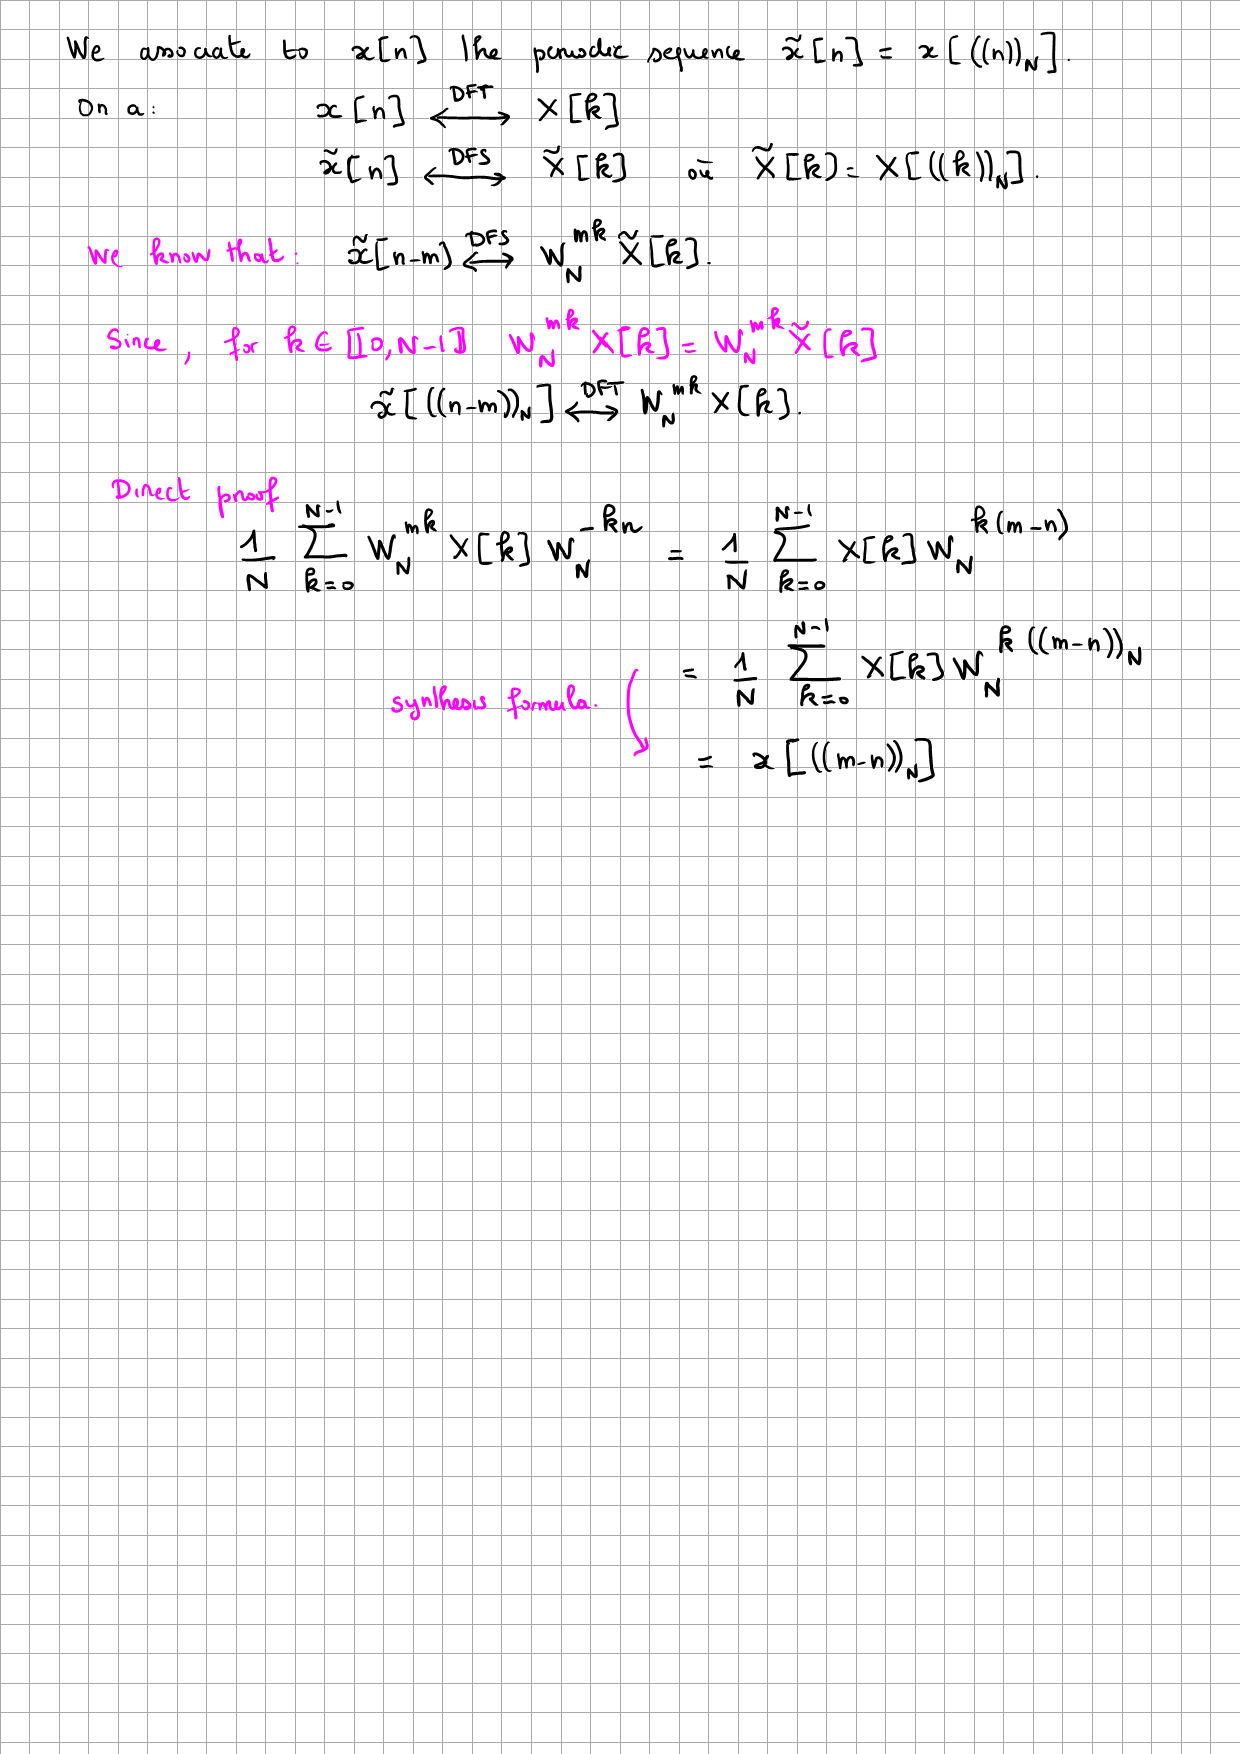
\includegraphics[width=\textwidth]{notecircularshift}}


\begin{frame}
\frametitle{Circular convolution}
\begin{itemize}
\item Consider two finite duration sequences $x_1[n]$ and $x_2[n]$, both of length $N$ and assume that $x_1[n] \ldft X_1[k]$ and $x_2[n] \ldft X_2[k]$. 
\item Set $X_3[k]= X_1[k]X_2[k]$ and 
\begin{align*}
x_3[n] 
&= \sum_{m=0}^{N-1} x_1[m] x_2[((n-m))_N] \\
&= \sum_{m=0}^{N-1} x_2[m] x_1[((n-m))_N]
\end{align*}
\item This operation is referred to a \alert{circular convolution}.
\end{itemize}
\end{frame}

\section{The Fast Fourier Transform}

\begin{frame}
\frametitle{Divide and Conquer: step 1}
\begin{figure}
  \centering
  % Requires \usepackage{graphicx}
  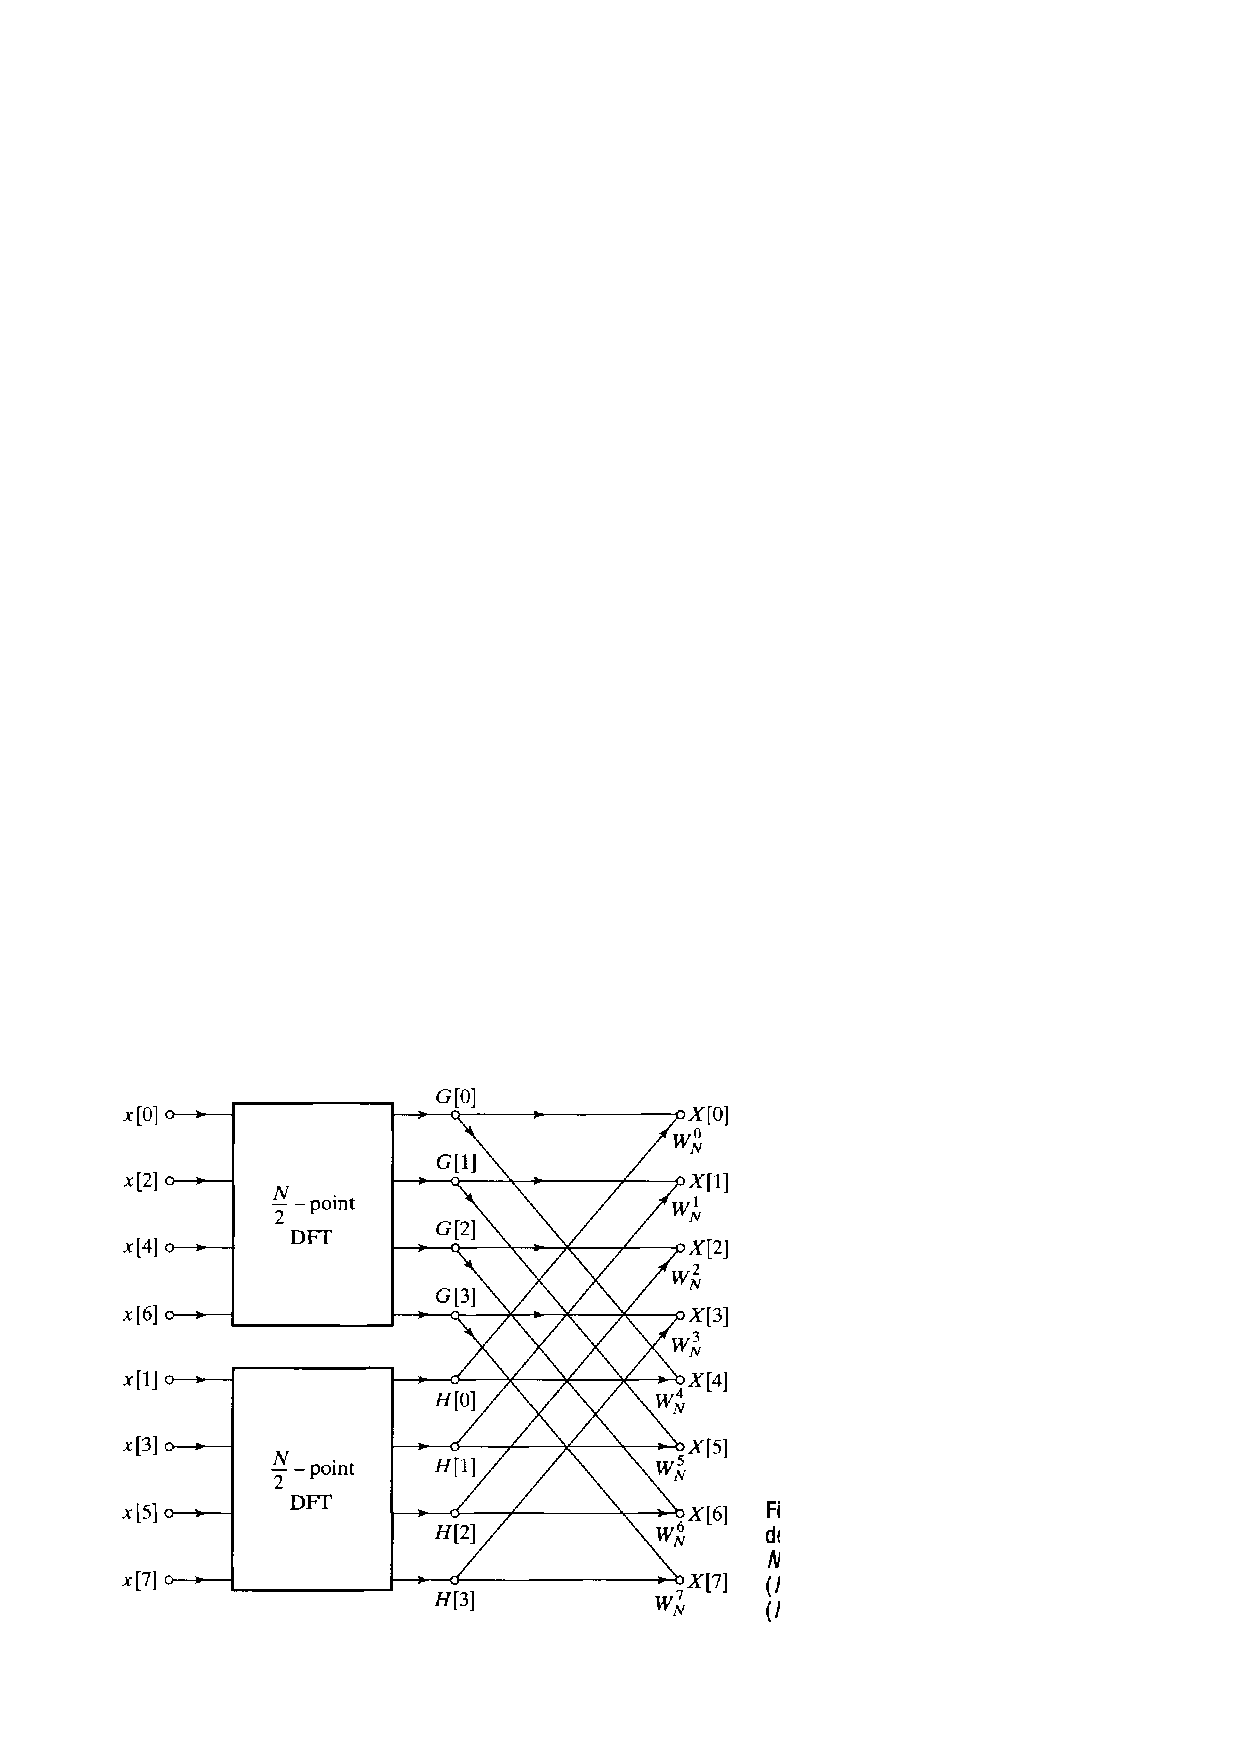
\includegraphics[width=0.7\textwidth]{FFT81}\\
\end{figure}

\end{frame}

\begin{frame}
\frametitle{Divide and Conquer: step 2}
\begin{figure}
  \centering
  % Requires \usepackage{graphicx}
  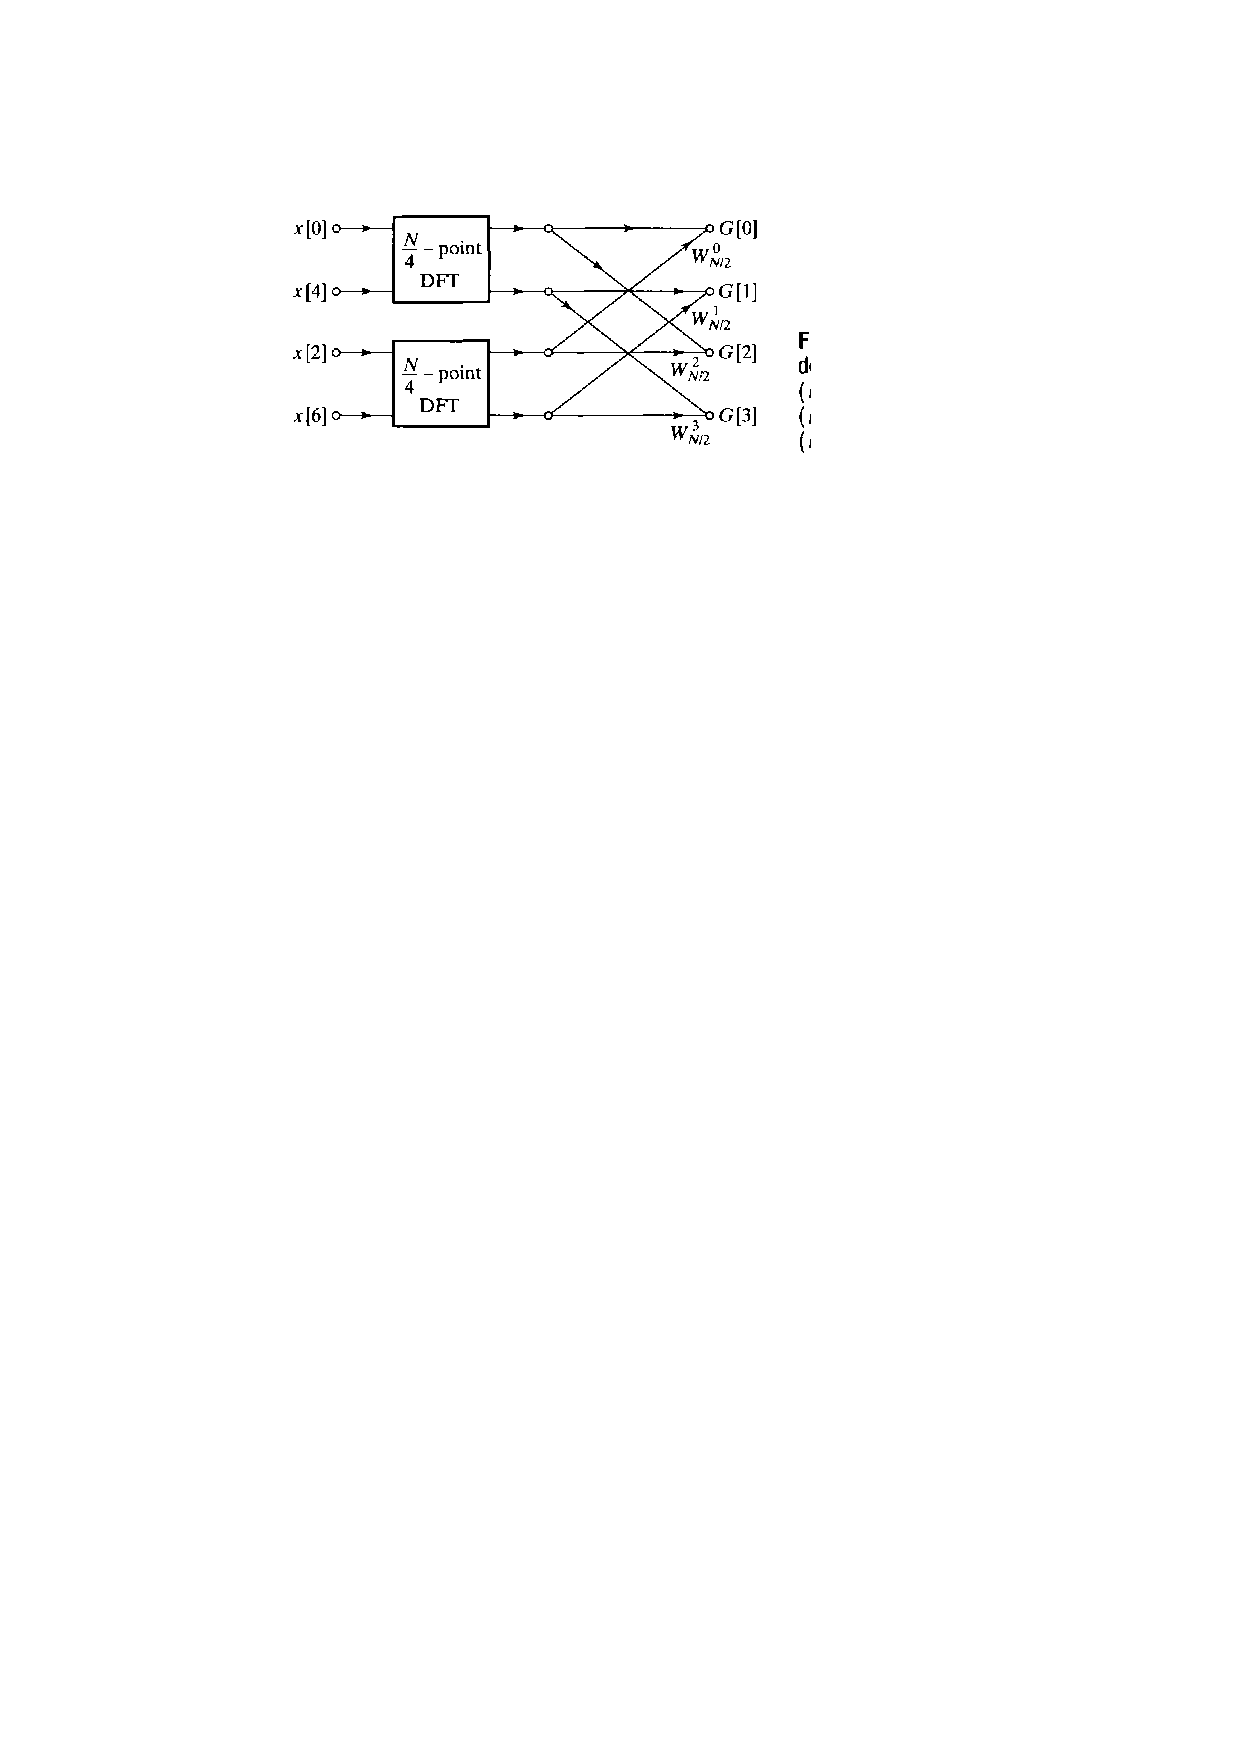
\includegraphics[scale=1]{FFT4}\\
\end{figure}
\end{frame}


\begin{frame}
\frametitle{Divide and Conquer: step 3}
\begin{figure}
  \centering
  % Requires \usepackage{graphicx}
  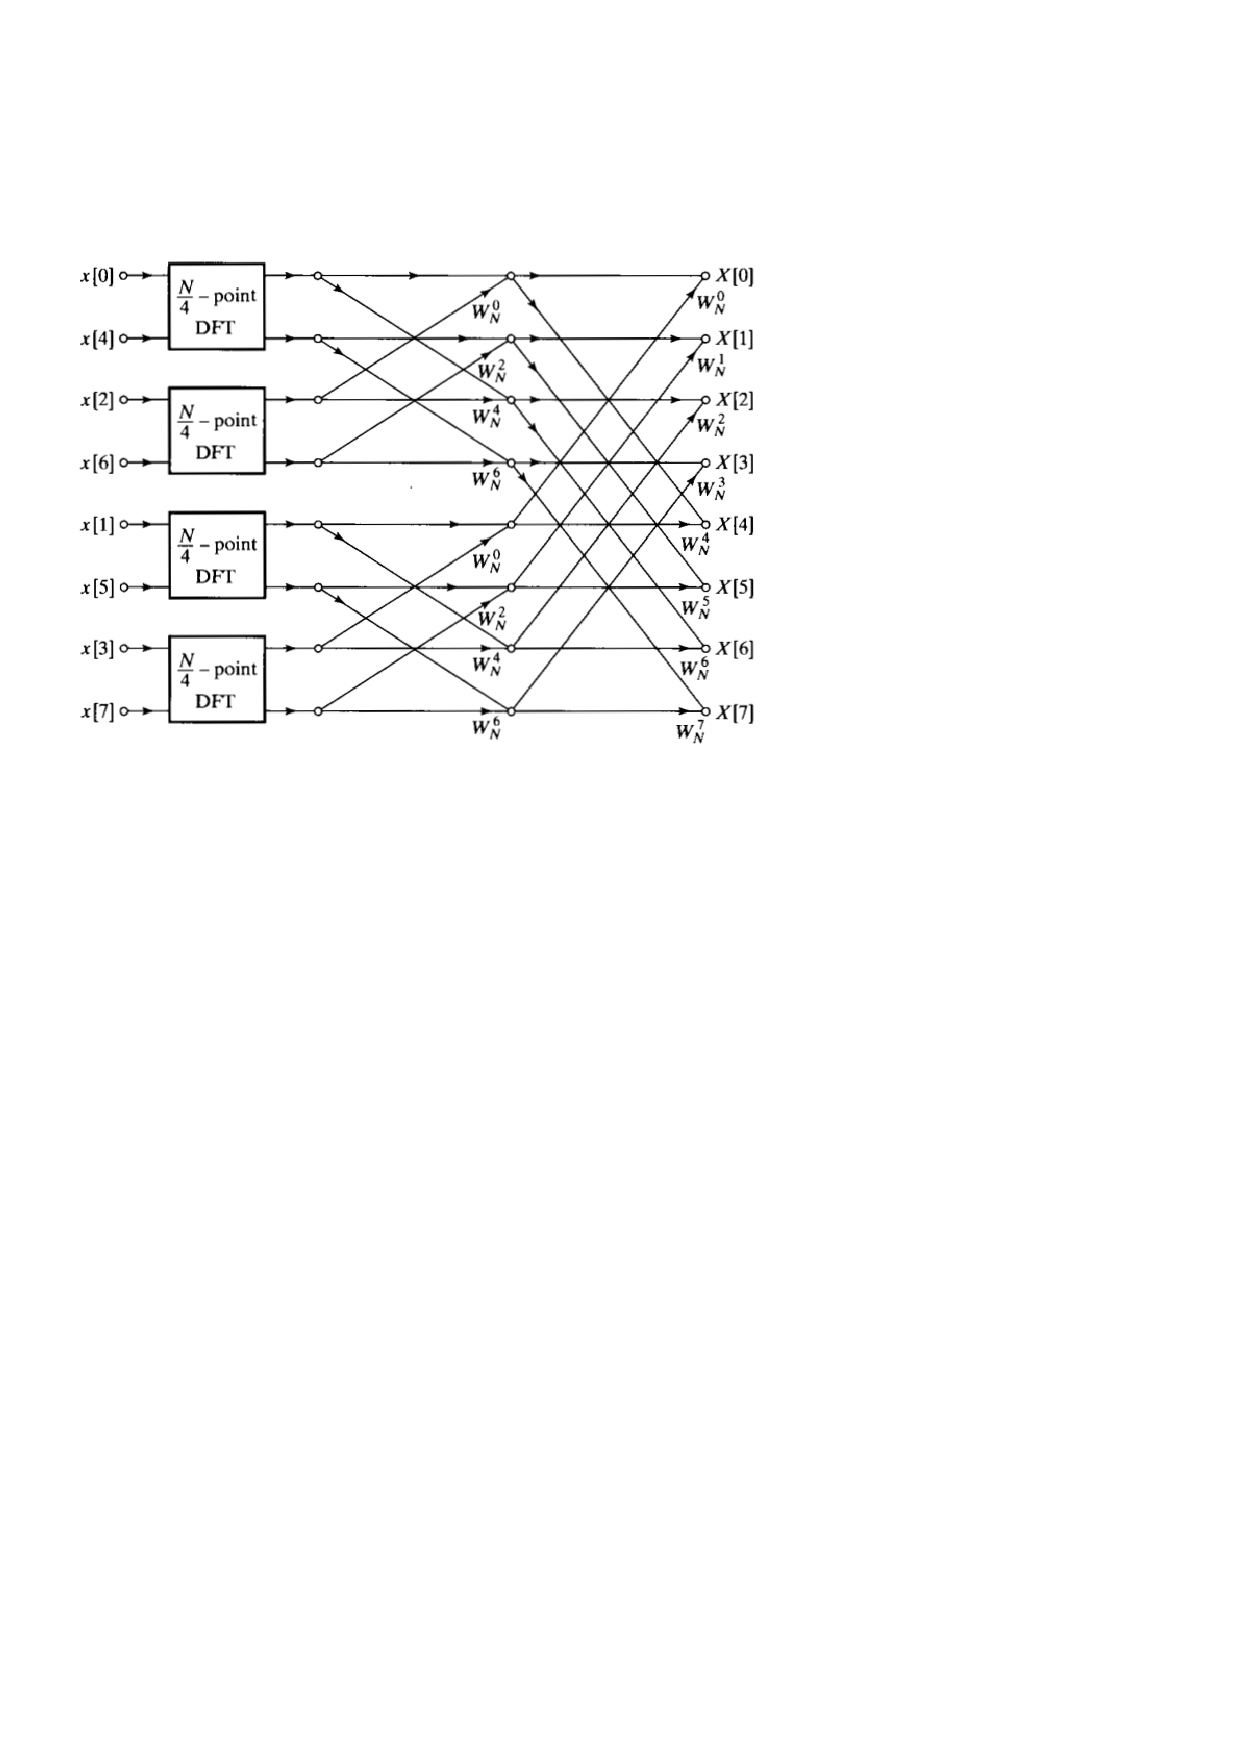
\includegraphics[width=0.7\textwidth]{FFT2stages}\\
\end{figure}
\end{frame}

\begin{frame}
\frametitle{FFT}
\begin{figure}
  \centering
  % Requires \usepackage{graphicx}
  \includegraphics[width=0.7\textwidth]{FFTfull}\\
\end{figure}
\end{frame}



\end{document} 